\documentclass[12pt, a4paper, oneside]{ctexart}
\usepackage{amsmath, amsthm, amssymb, bm, color, graphicx, geometry, mathrsfs,extarrows, braket, booktabs, array, xcolor, fontspec, appendix, float, subfigure, wrapfig}
\usepackage[colorlinks,linkcolor=red,anchorcolor=blue,citecolor=blue,urlcolor=blue,menucolor=black]{hyperref}

%%%% 设置英文字体 %%%%
\setmainfont{Times New Roman}
\setsansfont{Calibri}
\setmonofont{Consolas}

%%%% 设置代码块 %%%%
% 在vscode中使用minted需要先配置python解释器, Ctrl+Shift+P, 输入Python: Select Interpreter选择安装了Pygments的Python版本. 再在setting.json中xelatex和pdflatex的参数中加入 "--shell-escape", 即可
% TeXworks中配置方法参考: https://blog.csdn.net/RobertChenGuangzhi/article/details/108140093
\usepackage{minted}
\renewcommand{\theFancyVerbLine}{
    \sffamily\textcolor[rgb]{0.5,0.5,0.5}{\scriptsize\arabic{FancyVerbLine}}} % 修改代码前序号大小
\newmintinline{python}{linenos, breaklines, frame=lines, python3}  % 使用\pythoninline{代码}
\newminted{python}{linenos, breaklines, frame=lines, python3}  % 使用\begin{pythoncode}代码\end{pythoncode}
\newmintedfile{python}{linenos, breaklines, frame=lines, python3}  % 使用\pythonfile{代码地址}

%%%% 设置字号 %%%%
\newcommand{\chuhao}{\fontsize{42pt}{\baselineskip}\selectfont}     % 初号
\newcommand{\xiaochuhao}{\fontsize{36pt}{\baselineskip}\selectfont} % 小初号
\newcommand{\yihao}{\fontsize{28pt}{\baselineskip}\selectfont}      % 一号
\newcommand{\erhao}{\fontsize{21pt}{\baselineskip}\selectfont}      % 二号
\newcommand{\xiaoerhao}{\fontsize{18pt}{\baselineskip}\selectfont}  % 小二号
\newcommand{\sanhao}{\fontsize{15.75pt}{\baselineskip}\selectfont}  % 三号
\newcommand{\sihao}{\fontsize{14pt}{\baselineskip}\selectfont}      % 四号
\newcommand{\xiaosihao}{\fontsize{12pt}{\baselineskip}\selectfont}  % 小四号
\newcommand{\wuhao}{\fontsize{10.5pt}{\baselineskip}\selectfont}    % 五号
\newcommand{\xiaowuhao}{\fontsize{9pt}{\baselineskip}\selectfont}   % 小五号
\newcommand{\liuhao}{\fontsize{7.875pt}{\baselineskip}\selectfont}  % 六号
\newcommand{\qihao}{\fontsize{5.25pt}{\baselineskip}\selectfont}    % 七号

%%%% 设置行间距与页边距 %%%%
\linespread{1.3}
\geometry{left=2.5cm, right=2.5cm, top=2.5cm, bottom=2.5cm}

%%%% 定理类环境的定义 %%%%
\newtheorem{example}{例}            % 整体编号
\newtheorem{theorem}{定理}[section] % 定理按section编号
\newtheorem{definition}{定义}[section]
\newtheorem{axiom}{公理}[section]
\newtheorem{property}{性质}[section]
\newtheorem{proposition}{命题}[section]
\newtheorem{lemma}{引理}[section]
\newtheorem{corollary}{推论}[section]
\newtheorem{remark}{注解}
\newtheorem{condition}{条件}
\newtheorem{conclusion}{结论}
\newtheorem{assumption}{假设}
\newtheorem{algorithm}{算法}
\numberwithin{equation}{section}  % 公式按section编号 (公式右端的小括号)

%%%% 图片相对路径 %%%%
\graphicspath{{figure/}} % 当前目录下的figure文件夹, {../figure/}则是父目录的figure文件夹

\everymath{\displaystyle} % 默认全部行间公式, 想要变回行内公式使用\textstyle
\DeclareMathOperator*\uplim{\overline{lim}}     % 定义上极限 \uplim_{}
\DeclareMathOperator*\lowlim{\underline{lim}}   % 定义下极限 \lowlim_{}
\let\leq=\leqslant % 简写小于等于\leq (将全部leq变为leqslant)
\let\geq=\geqslant % 简写大于等于\geq (将全部geq变为geqslant)
\let\epsilon=\varepsilon % 简写\epsilon (将全部epsilon变为varepsilon)

%%%% 一些宏定义 %%%%%
\def\bd{\boldsymbol}        % 加粗(向量) boldsymbol
\def\disp{\displaystyle}    % 使用行间公式 displaystyle(默认)
\def\tsty{\textstyle}       % 使用行内公式 textstyle
\def\sign{\text{sign}}      % sign function
\def\wtd{\widetilde}        % 宽波浪线 widetilde
\def\R{\mathbb{R}}          % Real number
\def\N{\mathbb{N}}          % Natural number
\def\Z{\mathbb{Z}}          % Integer number
\def\C{\mathbb{C}}          % Complex number
\def\d{\mathrm{d}}          % differential operator
\def\e{\mathrm{e}}          % Euler's number
\def\i{\mathrm{i}}          % imaginary number
\def\re{\mathrm{Re}}        % Real part
\def\im{\mathrm{Im}}        % Imaginary part
\def\res{\mathrm{Res}}      % Residue
\def\L{\mathcal{L}}         % Loss function
\def\wdh{\widehat}          % 宽帽子 widehat
\def\ol{\overline}          % 上横线 overline
\def\ul{\underline}         % 下横线 underline
\def\add{\vspace{1ex}}      % 增加行间距
\def\del{\vspace{-3.5ex}}   % 减少行间距

%%%% 正文开始 %%%%
\begin{document}

%%%% 定义标题格式,包括title,author,affiliation,email等 %%%%
\title{素数定理的复分析证明}
\author{
吴天阳\\[1ex]
2204210460\\[1ex]
西安交通大学, 数学与统计学院, 强基数学002\\[1ex]
}
\date{\today}

\maketitle % 设置上面的标题

\begin{abstract}
    利用复分析完成素数定理证明, 将其分为以下5步完成: 先将素数定理转化为证明其充要条件, 转换到与$\psi_1$相关的证明上; 通过讨论Dirichlet级数的性质, 从而引出Riemann zeta函数的性质; 利用复积分的方法将$\psi_1$和zeta函数联系起来; 对zeta函数进行解析延拓, 使其成为在实部大于$0$的半平面上的亚纯函数; 对$G(s)$进行上界估计, 并证明zeta在直线$\re(s)=1$上无零点; 最终利用留数定理, 完成复分析证明.
    \add\add
    \textbf{关键字: }素数定理; Riemann zeta函数; 复分析; 留数定理
\end{abstract}
\clearpage % 创建新的一面
\tableofcontents % 创建目录,使用目录需要编译两次, 并且不能删去编译产生的临时文件!!!

%%%% 以下部分是正文 %%%%  
\clearpage

\CTEXsetup[format={\Large\bfseries}]{section}  % section靠左对齐
\section{素数定理介绍}
素数定理(Prime number theorem)描述的是素数在正整数中的渐进分布, 定理如下
\begin{equation}\label{eq-PNT}
    \lim_{x\to\infty}\frac{\pi(x)\log x}{x} = 1,
\end{equation}
其中$x\in \R$, $\pi(x)$表示小于等于$x$的素数个数.

Euler在1737年发现了著名的\textbf{Euler乘积公式}, 即
\begin{equation*}
    \zeta(s) = \sum_{n=1}^\infty\frac{1}{n^s} = \prod_p\frac{1}{1-p^{-s}}.
\end{equation*}

Carl Friedrich Gauss于1800年左右提出了有关素数定理的猜想. 在19世纪中期, Pafnuty Chebyshev发表了两篇重要的论文, 利用到了Euler乘积公式, 并且证明了如果(\ref{eq-PNT})的极限存在则一定为$1$.

Riemann在他著名的论文《论小于给定数值的素数个数》中破解了Euler乘积公式中与素数分布相关的信息, 为了纪念Riemann的贡献, 将Euler乘积公式左端的求和式称作Riemann zeta函数.

1896年, Jacques Hadamard和Charles Jean de la Vallée Poussin独立地证明了素数定理, 这两个证明都使用了zeta函数和复分析的方法.

1949年, Atle Selberg和Paul Erdős分别独立地证明了素数定理\cite{ref-elementary}, 他们的方法除了使用了极限, $e^x$, $\log x$的简单性质外, 没有涉及任何高等数学知识, 可以说是一个完全“初等”的证明.

后来于1980年, Donald J. Newman给出了一个近乎只用到Cauchy积分公式的简短证明\cite{ref-newman}, 1997年Don Zagier则将这证明压缩到三页纸.

本篇文章证明思路参考Ciar ́an O’Rourke的论文\cite{ref-three}, 该论文中具体介绍了三种证明素数定理的方法.
\subsection{一些约定和定义}
记$\N = \{1, 2, \cdots\}$, 即全体正整数. 对于没有具体声明的变量, 默认在正整数$\N$上取值, 例如$n \leq m$, 则$n$的取值为$\{1, 2,\cdots, m\}$; $n\geq m$, 则$n$的取值为$\{m, m+1,\cdots\}$. 如果没有特殊说明, 默认$p$取值为素数集合$\{2, 3, 5, 7, \cdots\}$.

在论文中, 对于复数$s\in \C$, 我们记$s = \sigma + it$, 其中$\sigma = \re(s),\ t = \im(s)$, \textbf{在文中出现$\sigma,\ t$都默认为复数$s$的实部和虚部}. 由Euler定理可知
\begin{equation*}
    |n^s| = |n^{\sigma +it}| = |e^{\sigma\log n}e^{it\log n}| = n^{\sigma}|e^{it\log n}| = n^{\sigma}.
\end{equation*}
\begin{definition}
    设$x\in\R$, 函数$[x]$的值为不大于$x$的最大整数, 函数$\{x\}$的值为$x - [x]$. 我们把$[x]$称为$x$的整数部分, $\{x\}$称为$x$的小数部分.
\end{definition}
\begin{definition}[整除]
    设$n,m$为整数, 若存在整数$k$, 使得$m = kn$, 则称$n$能整除$m$, 记为$n | m$; 否则, 称$n$不能整除$m$, 记为$n\nmid m$.
\end{definition}
\begin{definition}[渐进等价]
    设$f, g:\C\to\C$, 若
    \begin{equation*}
        \lim_{x\to\infty}\frac{f(x)}{g(x)} = 1,
    \end{equation*}
    则称当$x\to\infty$时, $f(x)$与$g(x)$渐近等价, 记做$f(x)\sim g(x)\quad (x\to\infty)$.
\end{definition}
于是素数定理又可以写为
\begin{equation*}
    \pi(x)\sim\frac{x}{\log x}\quad(x\to \infty).
\end{equation*}
下面我们会利用其它渐近等价作为素数定理的充要条件, 从而将素数定理转化为与复分析有关的问题.

\section{素数定理的充分性条件转化}
我们先将素数定理转化为证明其充分性定理, 先定义如下的三个对转化素数定理十分重要的函数.
\begin{definition}[Chebyshev第一函数]
    定义Chebyshev第一函数$\Theta:\R_{\geq 0}\to \R_{\geq 0}$如下
    \begin{equation*}
        \Theta(x) = \sum_{p\leq x}\log p.
    \end{equation*}
\end{definition}
不难发现$\Theta(x) = \sum_{p\leq x}\log p\leq \sum_{p\leq x}\log x = \pi(x)\log x$, 所以$\Theta$函数给出了素数定理的一个显然的下界, 而下面的Chebyshev第二函数给出了一个更加精确的下界.
\begin{definition}[von Mangoldt函数]
    定义von Mangoldt函数$\Lambda:\N\to\R$如下
    \begin{equation*}
        \Lambda = \begin{cases}
            \log p,&\quad n=p^r,\\
            0,&\quad \mathtt{otherwise}.
        \end{cases}
    \end{equation*}
\end{definition}
注意到$\Lambda$函数是从自然数集映射到复数域的子集, 我们将这样的函数称为$\textbf{数论函数}$. 这里顺便给出$\Lambda$函数的性质, 在后文中会用到.
\begin{proposition}\label{prop-lambda}
    任意$m\in \N$, 有
    \begin{equation*}
        \sum_{n|m}\Lambda(n) = \log m.
    \end{equation*}
\end{proposition}
\begin{proof}
    设$m$的标准分解式为$m = p_1^{\alpha_1}p_2^{\alpha_2}\cdots p_r^{\alpha_r}$, 于是
    \begin{equation*}
        \begin{aligned}
            \sum_{n|m}\Lambda(n) =&\ \sum_{k=1}^r\sum_{\beta=1}^{\alpha_k}\Lambda(p_k^{\beta}) = \sum_{k=1}^r\sum_{\beta=1}^{\alpha_k}\log p_k = \sum_{k=1}^r\alpha_k\log p_k = \sum_{k=1}^r\log p_k^{\alpha_k}\\
            =&\ \log(p_1^{\alpha_1}p_2^{\alpha_2}\cdots p_k^{\alpha_k}) = \log m.
        \end{aligned}
    \end{equation*}
\end{proof}
\begin{definition}[Chebyshev第二函数]
    定义Chebyshev第二函数$\psi:\R_{\geq 0}\to\R_{\geq 0}$如下
    \begin{equation*}
        \psi(x) = \sum_{n\leq x}\Lambda(n) = \sum_{k\geq 1}\sum_{p^k\leq x}\log p.
    \end{equation*}
\end{definition}
$\psi$函数对素数定理证明起到了至关重要的作用, 根据它的定义我们可以对$\pi(x)\log x$给出一个更精确的下界估计
\begin{equation*}
    \begin{aligned}
        \psi(x) =&\ \sum_{k\geq 1}\sum_{p^k\leq x}\log p = \sum_{p\leq x}\log p\sum_{p^k\leq x}1
        = \sum_{p\leq x}[\log_p x]\log p = \sum_{p\leq x}\left[\frac{\log x}{\log p}\right]\log p\\
        \leq&\ \sum_{p\leq x}\log x = \pi(x)\log x.
    \end{aligned}
\end{equation*}
由于$\psi(x) = \sum_{p\leq x}[\log_p x]\log p \geq \sum_{p\leq x}\log p = \Theta(x)$, 所以$\psi$相对于$\Theta$给出了一个更好的下界估计.
下面给出素数定理的一个充分性条件:
\begin{proposition}
    当$x\to\infty$时, 若$\psi(x)\sim x$成立, 则$\pi(x)\sim \frac{x}{x\log x}$.
\end{proposition}
\begin{proof}
    假设$\psi(x)\sim x$成立, 即对任意的$\epsilon > 0$, 存在充分大的$x$, 使得下式成立
    \begin{equation*}
        1-\epsilon\leq \frac{\psi(x)}{x}\leq 1+\epsilon.
    \end{equation*}
    
    取$\alpha \in (0,1)$, 则
    \begin{equation*}
        \psi(x)\geq\Theta(x) = \sum_{p\leq x}\log p\geq\sum_{x^{\alpha} < p\leq x}\log p\geq \sum_{x^{\alpha} < p\leq x}\log x^{\alpha} = \alpha(\pi(x)-\pi(x^{\alpha}))\log x,
    \end{equation*}
    于是, 当$x\to\infty$时
    \begin{equation*}
        \frac{\pi(x)\log x}{x}\leq \frac{\psi(x)}{\alpha x}+\frac{\pi(x^{\alpha})\log x}{x}\leq \frac{1}{\alpha}(1+\epsilon)+\frac{x^{\alpha}\log x}{x}=\frac{1}{\alpha}(1+\epsilon)+\frac{\log x}{x^{1-\alpha}}\to \frac{1}{\alpha}(1+\epsilon),
    \end{equation*}
    其中第二个等号是由$\pi(x^{\alpha})\leq x^{\alpha}$这个显然的估计得到的.\add

    令$\alpha = \frac{1}{1+\epsilon}$, 得
    \begin{equation*}
        1-\epsilon\leq \frac{\psi(x)}{x}\leq\frac{\pi(x)\log x}{x}\leq(1+\epsilon)^2,
    \end{equation*}
    所以$\pi(x)\sim\frac{x}{x\log x}\quad(x\to \infty)$.
\end{proof}
由于$\psi(x)$是非连续函数, 解析性质很差, 所以要引入一个光滑函数, 记
\begin{equation*}
    \psi_1(x) = \int_0^x\psi(u)\,\d u.
\end{equation*}

若$\psi(x)\sim x$, 猜测是否有$\psi_1(x) = \int_0^x \psi(u)\,\d u\sim \int_0^xu\,\d u = \frac{1}{2}x^2$, 于是又有以下充分性条件.
\begin{proposition}\label{prop-goto-psi1}
    当$x\to \infty$时, 若$\psi_1(x)\sim\frac{1}{2}x^2$成立, 则$\psi(x)\sim x$, 于是素数定理成立.
\end{proposition}
\begin{proof}
    由于$\psi(x)$是单调递增的, 对任意$x>0,\ \alpha \in (0, 1),\ \beta\in (1,\infty)$, 由积分第一中值定理知
    \begin{equation*}
        \begin{aligned}
            \frac{\psi_1(x)-\psi_1(\alpha x)}{(1-\alpha)x^2} \leq \frac{1}{x(x-\alpha x)}&\int_{\alpha x}^x\psi(u)\,\d u\leq \frac{\psi(x)}{x}\\
            &\qquad\qquad\leq \frac{1}{x(\beta x - x)}\int_x^{\beta x}\psi(u)\,\d u = \frac{\psi_1(\beta x)-\psi_1(x)}{(\beta -1)x^2}.
        \end{aligned}
    \end{equation*}

    假设当$x\to \infty$时, $\psi_1(x)\sim \frac{1}{2}x^2$, 于是
    \begin{equation*}
        \begin{aligned}
            &\ \frac{\psi_1(x)-\psi_1(\alpha x)}{(1-\alpha)x^2}\sim \frac{(1-\alpha^2)x^2}{2(1-\alpha)x^2} = \frac{1+\alpha}{2},\\
            &\ \frac{\psi_1(\beta x)-\psi_1(x)}{(\beta -1)x^2}\sim \frac{(\beta^2-1)x^2}{2(\beta - 1)x^2} = \frac{\beta+1}{2}.
        \end{aligned}
    \end{equation*}

    对于任意$\epsilon > 0$, 存在充分大的$x$使得
    \begin{equation*}
        \frac{1+\alpha}{2}(1-\epsilon)\leq \frac{\psi_1(x)-\psi_1(\alpha x)}{(1-\alpha)x^2},\quad\frac{\psi_1(\beta x)-\psi_1(x)}{(\beta-1)x^2} \leq \frac{\beta+1}{2}(1+\epsilon),
    \end{equation*}
    则有
    \begin{equation*}
        \frac{1+\alpha}{2}(1-\epsilon)\leq \frac{\psi(x)}{x}\leq \frac{\beta+1}{2}(1+\epsilon).
    \end{equation*}

    取$\alpha = 1-2\epsilon,\ \beta = 1+2\epsilon$, 得
    \begin{equation*}
        (1-\epsilon)^2\leq \frac{\psi(x)}{x}\leq (1+\epsilon)^2,
    \end{equation*}
    所以$\psi(x)\sim x\quad (x\to \infty)$.
\end{proof}
于是我们又得到一个素数定理的充分性条件, 而且$\psi_1$具有很好的解析性质, 我们知道$\psi$和$\Lambda$有关联, 所以$\psi_1(x)$应该也可与$\Lambda$找到联系.
\begin{proposition}\label{prop-psi-lambda}
    对任意$x \geq 1$, 有$\psi_1(x)=\sum_{n\leq x}\Lambda(n)(x-n)$.
\end{proposition}
\begin{proof}
    由于
    \begin{equation*}
        \psi_1(x) = \int_0^x\psi(u)\,\d u = \int_0^x\sum_{n\leq u}\Lambda(u)\,\d u = \int_0^x\sum_{n=1}^\infty \Lambda(n)f_n(u)\,\d u,
    \end{equation*}
    其中$f_n(u) = \begin{cases}
        1,&\quad n\leq u,\\
        0,&\quad \mathtt{otherwise}.
    \end{cases}$

    则
    \begin{equation*}
        \psi_1(x) = \sum_{n=1}^\infty\Lambda(n)\int_0^xf_n(u)\,\d u =\sum_{n\leq x}\Lambda(n)\int_n^x\,\d u= \sum_{n\leq x}\Lambda(n)(x-n).
    \end{equation*}
\end{proof}
接下来我们先讨论Dirichlet级数性质, 再取其特例得到Riemann zeta函数的性质.
\section{Dirichlet级数与zeta函数}
设$s\in\C$, 记$s = \sigma + it$, 其中$\sigma = \re(s),\ t = \im(s)$.
\begin{definition}[Dirichlet级数]设数论函数$f:\N\to\C$, 定义Dirichlet级数如下
    \begin{equation*}
        F(s) = \sum_{n=1}^\infty\frac{f(n)}{n^s} \quad(s\in \C).
    \end{equation*}
\end{definition}
\begin{definition}[Riemann zeta函数]一种Dirichlet级数, 取$f(n) = 1$, 记
    \begin{equation*}
        \zeta(s) = \sum_{n=1}^\infty\frac{1}{n^s}\quad(\sigma > 1).
    \end{equation*}
    其中$\sigma$为复数$s$的实部. 将$\zeta(s)$称为Riemann zeta函数, 简称为zeta函数.
\end{definition}
这一节我们将给出zeta函数和$\Lambda$函数的关系, 为下一节建立$\psi_1$和$\zeta$函数的关系做准备. 我们先讨论Dirichlet级数的性质, 再特值$f(n)=1$, 从而转化到zeta函数上. 首先给出Dirichlet级数收敛性条件, 证明请见\cite{ref-复变函数}第5章定理6.
\begin{theorem}\label{thm-dirichlet}
    任一Dirichlet级数$F(s)$都有一收敛直线$\sigma = c$, 满足:
    
    (1) 级数在直线的右半平面收敛, 在直线的左半平面内发散;

    (2) 级数在收敛直线的右半平面内内闭一致收敛.

    且存在以收敛直线$\sigma = c' > c$, 使得Dirichlet级数在直线的右半平面内绝对收敛.
\end{theorem}
\begin{proposition}
    假设存在三个Dirichlet级数
    \begin{equation*}
        F_j(s) = \sum_{n=1}^\infty\frac{f_j(n)}{n^s}\quad(j=1,2,3),
    \end{equation*}
    满足任意$n\in \N$, 有
    \begin{equation*}
        f_3(n) = \sum_{m_1m_2= n}f_1(m_1)f_2(m_2).
    \end{equation*}

    设$F_j(s)$分别在$\sigma > \sigma_j\ (j=1,2)$上绝对收敛, 当$\sigma > \max\{\sigma_1, \sigma_2\}$时
    \begin{equation*}
        F_3(s) = F_1(s)F_2(s),
    \end{equation*}
\end{proposition}
\begin{proof}
    由于
    \begin{equation*}
        \begin{aligned}
            \sum_{n=1}^N\frac{f_3(n)}{n^s} =&\ \sum_{n=1}^N\sum_{m_1m_2 = n}\frac{f_1(m_1)f_2(m_2)}{n^s} = \sum_{n=1}^N\sum_{m_1m_2=n} \frac{f_1(m_1)}{m_1^s}\,\frac{f_2(m_2)}{m_2^s}\\
            =&\ \sum_{m_1\leq N}\sum_{m_2\leq N/m_1}\frac{f_1(m_1)}{m_1^s}\,\frac{f_2(m_2)}{m_2^s}\\
            =&\ \sum_{m_1\leq \sqrt{N}}\frac{f_1(m_1)}{m_1^s}\sum_{m_2\leq N/m_1}\frac{f_2(m_2)}{m_2^s}+\sum_{\sqrt{N}<m_1\leq N}\frac{f_1(m_1)}{m_1^s}\sum_{m_2\leq N/m_1}\frac{f_2(m_2)}{m_2^s}.
        \end{aligned}
    \end{equation*}
    因此
    \begin{equation*}
        \begin{aligned}
            \sum_{n=1}^N\frac{f_3(n)}{n^s}-&\ \sum_{m_1\leq \sqrt{N}}\frac{f_1(m_1)}{m_1^s}\sum_{m_2\leq \sqrt{N}}\frac{f_2(m_2)}{m_2^s}\\
            &\ =\sum_{m_1\leq \sqrt{N}}\frac{f_1(m_1)}{m_1^s}\sum_{\sqrt{N} < m_2\leq N/m_1}\frac{f_2(m_2)}{m_2^s}+\sum_{\sqrt{N}<m_1\leq N}\frac{f_1(m_1)}{m_1^s}\sum_{m_2\leq N/m_1}\frac{f_2(m_2)}{m_2^s},
        \end{aligned}
    \end{equation*}
    于是
    \begin{equation*}
        \begin{aligned}
            &\ \left|\sum_{n=1}^N\frac{f_3(n)}{n^s} -\sum_{m_1\leq \sqrt{N}}\frac{f_1(m_1)}{m_1^s}\sum_{m_2\leq \sqrt{N}}\frac{f_2(m_2)}{m_2^s}\right| \\
            \leq&\ \sum_{m_1\leq \sqrt{N}}\left|\frac{f_1(m_1)}{m_1^s}\right|\sum_{\sqrt{N} < m_2\leq N/m_1}\left|\frac{f_2(m_2)}{m_2^s}\right|+\sum_{\sqrt{N}<m_1\leq N}\left|\frac{f_1(m_1)}{m_1^s}\right|\sum_{m_2\leq N/m_1}\left|\frac{f_2(m_2)}{m_2^s}\right|\\
            \leq&\ \sum_{m_1=1}^\infty\left|\frac{f_1(m_1)}{m_1^s}\right|\sum_{m_2 > \sqrt{N}}\left|\frac{f_2(m_2)}{m_2^s}\right|+\sum_{m_1>\sqrt{N}}\left|\frac{f_1(m_1)}{m_1^s}\right|\sum_{m_2=1}^\infty\left|\frac{f_2(m_2)}{m_2^s}\right|\\
            =&\ F_1(s)\sum_{m_2>\sqrt{N}}\left|\frac{f_2(m_2)}{m_2^s}\right|+F_2(s)\sum_{m_1>\sqrt{N}}\left|\frac{f_1(m_1)}{m_1^s}\right|\to 0\quad(N\to \infty).
        \end{aligned}
    \end{equation*}
    由于当$\sigma > \max\{\sigma_1,\sigma_2\}$时, $F_1(s),\ F_2(s)$均绝对收敛, 所以当$n\to \infty$时, 上式趋于$0$.

    综上
    \begin{equation*}
        F_1(s) = \sum_{1}^\infty\frac{f_3(n)}{n^s}=\sum_{m_1=1}^\infty\frac{f_1(m_1)}{m_1^s}\sum_{m_2=1}^\infty\frac{f_2(m_2)}{m_2^s} = F_2(s)F_3(s).
    \end{equation*}
\end{proof}
由归纳法不难得出以下推论.
\begin{corollary}
\label{corollary-乘积}
    假设存在$k+1\ (k\geq 2)$个Dirichlet级数
    \begin{equation*}
        F_j(s)=\sum_{n=1}^\infty\frac{f_j(n)}{n^s},
    \end{equation*}
    且满足对任意$n\in \N$有
    \begin{equation*}
        f_{k+1}(n) = \sum_{m_1m_2\cdots m_k=n}f_1(m_1)f_2(m_2)\cdots f_k(m_k).
    \end{equation*}

    设$F_j(s)$分别在$\sigma > \sigma_j\ (j=1,2,\cdots, k)$上绝对收敛, 当$\sigma > \max\{\sigma_1,\sigma_2,\cdots, \sigma_k\}$时
    \begin{equation*}
        F_{k+1}(s) = F_1(s)F_2(s)\cdots F_k(s).
    \end{equation*}
\end{corollary}
\begin{proposition}\label{prop-prod}
    设函数$f:\N\to \C$是完全积性函数, 即对任意整数$n,m$都有$f(nm) = f(n)f(m)$成立. 若Dirichlet级数
    \begin{equation*}
        F(s) = \sum_{n=1}^\infty\frac{f(n)}{n^s}
    \end{equation*}
    绝对收敛, 则
    \begin{equation*}
        F(s) = \prod_{p}\sum_{\alpha =0}^\infty\frac{f(p^\alpha)}{p^{\alpha s}}.
    \end{equation*}
\end{proposition}
\begin{proof}
    设$p_j$表示从小到大第$j$个素数, 定义数论函数$g_j:\N\to\C$如下
    \begin{equation*}
        g_j(n) = \begin{cases}
            f(n),&\quad p_j|n\ \text{或}\ n=1,\\
            0,&\quad\mathtt{otherwise}.
        \end{cases}
    \end{equation*}
    由\textbf{推论}\ref{corollary-乘积}可知
    \begin{equation}\label{eq-prod-1}
        \sum_{n=1}^\infty\sum_{m_1m_2\cdots m_k=n}g_1(m_1)g_2(m_2)\cdots g_k(m_k)n^{-s} = \prod_{j=1}^k\sum_{n=1}^\infty\frac{g_j(n)}{n^s},
    \end{equation}
    且
    \begin{equation}\label{eq-prod-2}
        \sum_{n=1}^\infty\frac{g_j(n)}{n^s}=\sum_{\substack{n=p_j^\alpha\\\alpha \geq 0}}\frac{g_j(n)}{n^s}=\sum_{\substack{n=p_j^\alpha\\\alpha \geq 0}}\frac{f(n)}{n^s}=\sum_{\alpha = 0}^\infty\frac{f(p_j^\alpha)}{p_j^{\alpha s}},
    \end{equation}
    考虑求和式$S_n = \sum_{m_1m_2\cdots m_k = n}g_1(m_1)g_2(m_2)\cdots g_k(m_k)$, 下面分两种情况讨论$n$.

    当$n=p_1^{\alpha_1}p_2^{\alpha_2}\cdots p_k^{\alpha_k}$, 其中$\alpha_k \geq 0\ (j=1,2,\cdots, k)$, 令$m_j = p_j^{\alpha_j}$, 于是$n = m_1m_2\cdots m_k$, 则
    \begin{equation*}
        S_n = f(p_1^{\alpha_1})f(p_2^{\alpha_2})\cdots f(p_k^{\alpha_k}) = f(p_1^{\alpha_1}p_2^{\alpha_2}\cdots p_k^{\alpha_k}) = f(n).
    \end{equation*}

    当$n = p_1^{\alpha _1}p_2^{\alpha_2}\cdots p_k^{\alpha_k}q^{\beta}\ (p_j\nmid q, j=1,2,\cdots, k, \beta > 0)$, 则$n \neq m_1m_2\cdots m_k$, 所以$S_n = 0$.

    因此
    \begin{equation}\label{eq-prod-3}
        S_n =\sum_{m_1m_2\cdots m_k = n}g_1(m_1)g_2(m_2)\cdots g_k(m_k) = \theta_k(n)f(n),
    \end{equation}
    其中$\theta_k(n) = \begin{cases}
        1,&\quad n=p_1^{\alpha_1}p_2^{\alpha_2}\cdots p_k^{\alpha_k},\ \alpha_1,\alpha_2,\cdots,\alpha_k\geq 0,\\
        0,&\quad \mathtt{otherwise}.
    \end{cases}$\add

    由(\ref{eq-prod-1}), (\ref{eq-prod-2}), (\ref{eq-prod-3})式可知
    \begin{equation*}
        \prod_{j=1}^k\sum_{\alpha=0}^\infty\frac{f(p_j^{\alpha})}{p_j^{\alpha s}} = \sum_{n=1}^\infty\theta_k(n)\frac{f(n)}{n^s},
    \end{equation*}
    于是
    \begin{equation*}
        \prod_{j=1}^k\sum_{\alpha=0}^\infty\frac{f(p_j^{\alpha})}{p_j^{\alpha s}} -\sum_{n=1}^\infty\frac{f(n)}{n^s} = \sum_{n=1}^\infty(\theta_k(n)-1)\frac{f(n)}{n^s}.
    \end{equation*}

    由于$k\leq p_k$, 当$n\leq k$时, $n\leq p_k$, 于是$\theta_k(n) - 1 = 0$, 因此
    \begin{equation*}
        \left|\prod_{j=1}^k\sum_{\alpha=0}^\infty\frac{f(p_j^{\alpha})}{p_j^{\alpha s}}-F(s)\right|=\left|\sum_{n=k+1}^\infty(\theta_k(n)-1)\frac{f(n)}{n^s}\right|\leq \sum_{n=k+1}^\infty\left|\frac{f(n)}{n^{s}}\right|\to 0\quad(k\to \infty),
    \end{equation*}
    由于$F(s)$绝对收敛, 所以当$k\to\infty$时, 上式趋于$0$.

    综上
    \begin{equation*}
        F(s) = \prod_{j=1}^\infty\sum_{\alpha=0}^\infty\frac{f(p_j^{\alpha})}{p_j^{\alpha s}} = \prod_p\sum_{\alpha = 0}^\infty\frac{f(p^{\alpha})}{p^{\alpha s}}.
    \end{equation*}
\end{proof}
\begin{proposition}\label{prop-prod-series}
    设函数$f:\N\to \C$是完全积性函数且不为$0$, 若Dirichlet级数
    \begin{equation*}
        F(s)=\sum_{n=1}^\infty\frac{f(n)}{n^s}
    \end{equation*}
    绝对收敛, 则
    \begin{equation*}
        F(s) = \prod_s\frac{1}{1-\frac{f(p)}{p^s}}.
    \end{equation*}
\end{proposition}
\begin{proof}
    考虑级数
    \begin{equation*}
        G_p(s) = \sum_{\alpha = 0}^\infty\frac{f(p^\alpha)}{p^{\alpha s}},
    \end{equation*}
    因此
    \begin{equation*}
        G_p(s) = \sum_{\alpha = 0}^\infty \frac{f(p^{\alpha})}{p^{\alpha s}} = \sum_{n= p^{\alpha}}\frac{f(n)}{n^s},
    \end{equation*}
    所以$G_p(s)$是$F(s)$的子序列, 于是$G(s)$绝对收敛.

    利用$f(n)$是完全积性函数且不为$0$, 知
    \begin{equation*}
        G_p(s) = \sum_{\alpha = 0}^{\infty}\frac{f(p^{\alpha})}{p^{\alpha s}} = \sum_{\alpha =0}^\infty\left(\frac{f(p)}{p^s}\right)^{\alpha} = \frac{1}{1-\frac{f(p)}{p^s}}.
    \end{equation*}

    由\textbf{命题}\ref{prop-prod}知
    \begin{equation*}
        F(s) = \prod_p G_p(s) = \prod_p\frac{1}{1-\frac{f(p)}{p^s}}.
    \end{equation*}
\end{proof}
注意到$f(n) = 1$是完全积性函数, 所以由\textbf{命题}\ref{prop-prod-series}, 我们可以得到所谓的\textbf{Euler乘积公式}
\begin{equation}\label{eq-zeta-prod}
    \zeta(s) = \prod_p\frac{1}{1-\frac{1}{p^s}}\quad(\sigma > 1).
\end{equation}
\begin{proposition}\label{prop-zeta-zero1}
    当$\sigma > 1$时, 即$\re(s) > 1$, 则$\zeta(s)\neq 0$.
\end{proposition}
\begin{proof}
    由(\ref{eq-zeta-prod})式可知
    \begin{equation*}
        |\zeta(s)| = \left|\prod_p\frac{1}{1-\frac{1}{p^s}}\right|=\prod_p\frac{1}{\left|1-\frac{1}{p^s}\right|},
    \end{equation*}
    又由于
    \begin{equation*}
        \left|1-\frac{1}{p^s}\right| = |1-p^{-\sigma-i t}| \leq 1+|p^{-\sigma-it}| = 1+p^{-\sigma},
    \end{equation*}
    于是
    \begin{equation}\label{eq-zeta-zero1}
        |\zeta(s)|=\prod_p\frac{1}{\left|1-\frac{1}{p^s}\right|}\geq \prod_p\frac{1}{1+p^{-a}} = \prod_p\frac{1-p^{-a}}{1-p^{-2a}} = \prod_p\frac{(1-p^{-2a})^{-1}}{(1-p^{-a})^{-1}}=\frac{\zeta(2a)}{\zeta(a)} > 0.
    \end{equation}
\end{proof}
\begin{theorem}[Weierstrass]\label{thm-weierstrass}
    若函数序列$f_n(z)\ (n=1,2,\cdots)$在区域$D$内解析, 级数$\sum_{n=1}^\infty f_n(z)$在$D$内内闭一致收敛到函数$f(z)$, 则
    
    (1) 函数$f(z)$在$D$内解析;
    
    (2) 级数$\sum_{n=1}^\infty f_n^{(k)}(z)$在$D$内内闭一致收敛到$f^{(k)}(z),\ k\in\N$.
\end{theorem}
证明请见\cite{ref-复变函数}第5章定理3.\add

由于$\zeta(s)=\sum_{n=1}^\infty\frac{1}{n^s}$在$s = x > 1\ (x\in \R)$上收敛\footnote{证明请见\cite{ref-数分}第九章例1.9.}, 由\textbf{定理}\ref{thm-dirichlet}知, $\zeta(s)$在区域$D = \{\sigma = \re(s) >1\}$上一致收敛, 又由于$\frac{1}{n^s}$在$D$上解析, 由\textbf{定理}\ref{thm-weierstrass}可知, $\zeta(s)$在$D$上解析, 且
\begin{equation}\label{eq-zeta-diff}
    \zeta'(s) = -\sum_{n=1}^\infty\frac{\log n}{n^s}.
\end{equation}
\begin{proposition}\label{prop-zeta-lambda}
    设$\sigma > 1$, 即$\re(s) > 1$, 则
    \begin{equation*}
        -\frac{\zeta'(s)}{\zeta(s)}=\sum_{n=1}^\infty\frac{\Lambda(n)}{n^s}.
    \end{equation*}
\end{proposition}
\begin{proof}
    设$\sigma = \re(s) > 0$, 由\textbf{命题}\ref{prop-zeta-zero1}知$\zeta(s)\neq 0$, 注意到\textbf{命题}\ref{prop-lambda}
    \begin{equation}\label{eq-lambda}
    \log_n = \sum_{m|n}\Lambda(m) = \sum_{m_1m_2 = n}\Lambda(m_1)\mathbf{1}(m_2),
    \end{equation}
    其中$\mathbf{1}(n) = 1\ (n\in\N)$为常值函数.
    
    由于
    \begin{equation*}
        \left|\sum_{n=1}^\infty\frac{\Lambda(n)}{n^s}\right|=\sum_{n=1}^\infty\frac{\Lambda(n)}{n^{\sigma}}\leq\sum_{n=1}^\infty\frac{\log n}{n^\sigma} < \infty\quad(\sigma > 1),
    \end{equation*}
    于是当$\sigma > 0$时, $\sum_{n=1}^\infty\frac{\Lambda(n)}{n^s}$收敛.

    由\textbf{命题}\ref{prop-prod}和(\ref{eq-zeta-prod}), (\ref{eq-zeta-diff}), (\ref{eq-lambda})式知
    \begin{equation*}
        -\zeta'(s) = \sum_{n=1}^\infty\frac{\log n}{n^s} = \sum_{n=1}^\infty\frac{\Lambda(n)}{n^s}\sum_{n=1}^\infty\frac{u(n)}{n^s} = \sum_{n=1}^\infty\frac{\Lambda(n)}{n^s}\sum_{n=1}^\infty\frac{1}{n^s} = \zeta(s)\sum_{n=1}^\infty\frac{1}{n^s},
    \end{equation*}
    所以
    \begin{equation*}
        -\frac{\zeta'(s)}{\zeta(s)}=\sum_{n=1}^\infty\frac{\Lambda(n)}{n^s}.
    \end{equation*}
\end{proof}
\section{\texorpdfstring{$\psi_1(x)$}{}的复积分形式}
\begin{lemma}\label{le-psi}
    设$a >0$且$c>1$, 则
    \begin{equation*}
        \frac{1}{2\pi \i}\int_{c-i\infty}^{c+i\infty}\frac{a^s}{s(s+1)}\,\d s=\begin{cases}
            0,&\quad0 < a\leq 1,\\
            1-\frac{1}{a},&\quad a \geq 1.
        \end{cases}
    \end{equation*}
\end{lemma}
\begin{proof}
    设$f(s) = \frac{a^s}{s(s+1)}$, 下面分别根据$a$的不同取值范围构造不同的曲线, 再使用留数定理进行证明.
    
    当$a\geq 1$时, 构造圆弧$A(T) = \{s:|s|\leq \sqrt{c^2+T^2},\ \sigma < c\}$, \add 直线段$B(T) = [c-\i T, c+\i T]$, 设$\gamma(T) = A(T) \cup B(T)$定向为逆时针方向, 则$\gamma(T)$为简单闭合曲线, 且包含$\frac{a^s}{s(s+1)}$的两个一级极点$s=0,-1$. 如\textbf{图}\ref{figure-psi1}所示.
    \begin{figure}[htbp] % h: 当前位置, t: 顶部, b: 底部, p: 浮动页, 这样组合指的是使用这个顺序进行排版
        \centering
        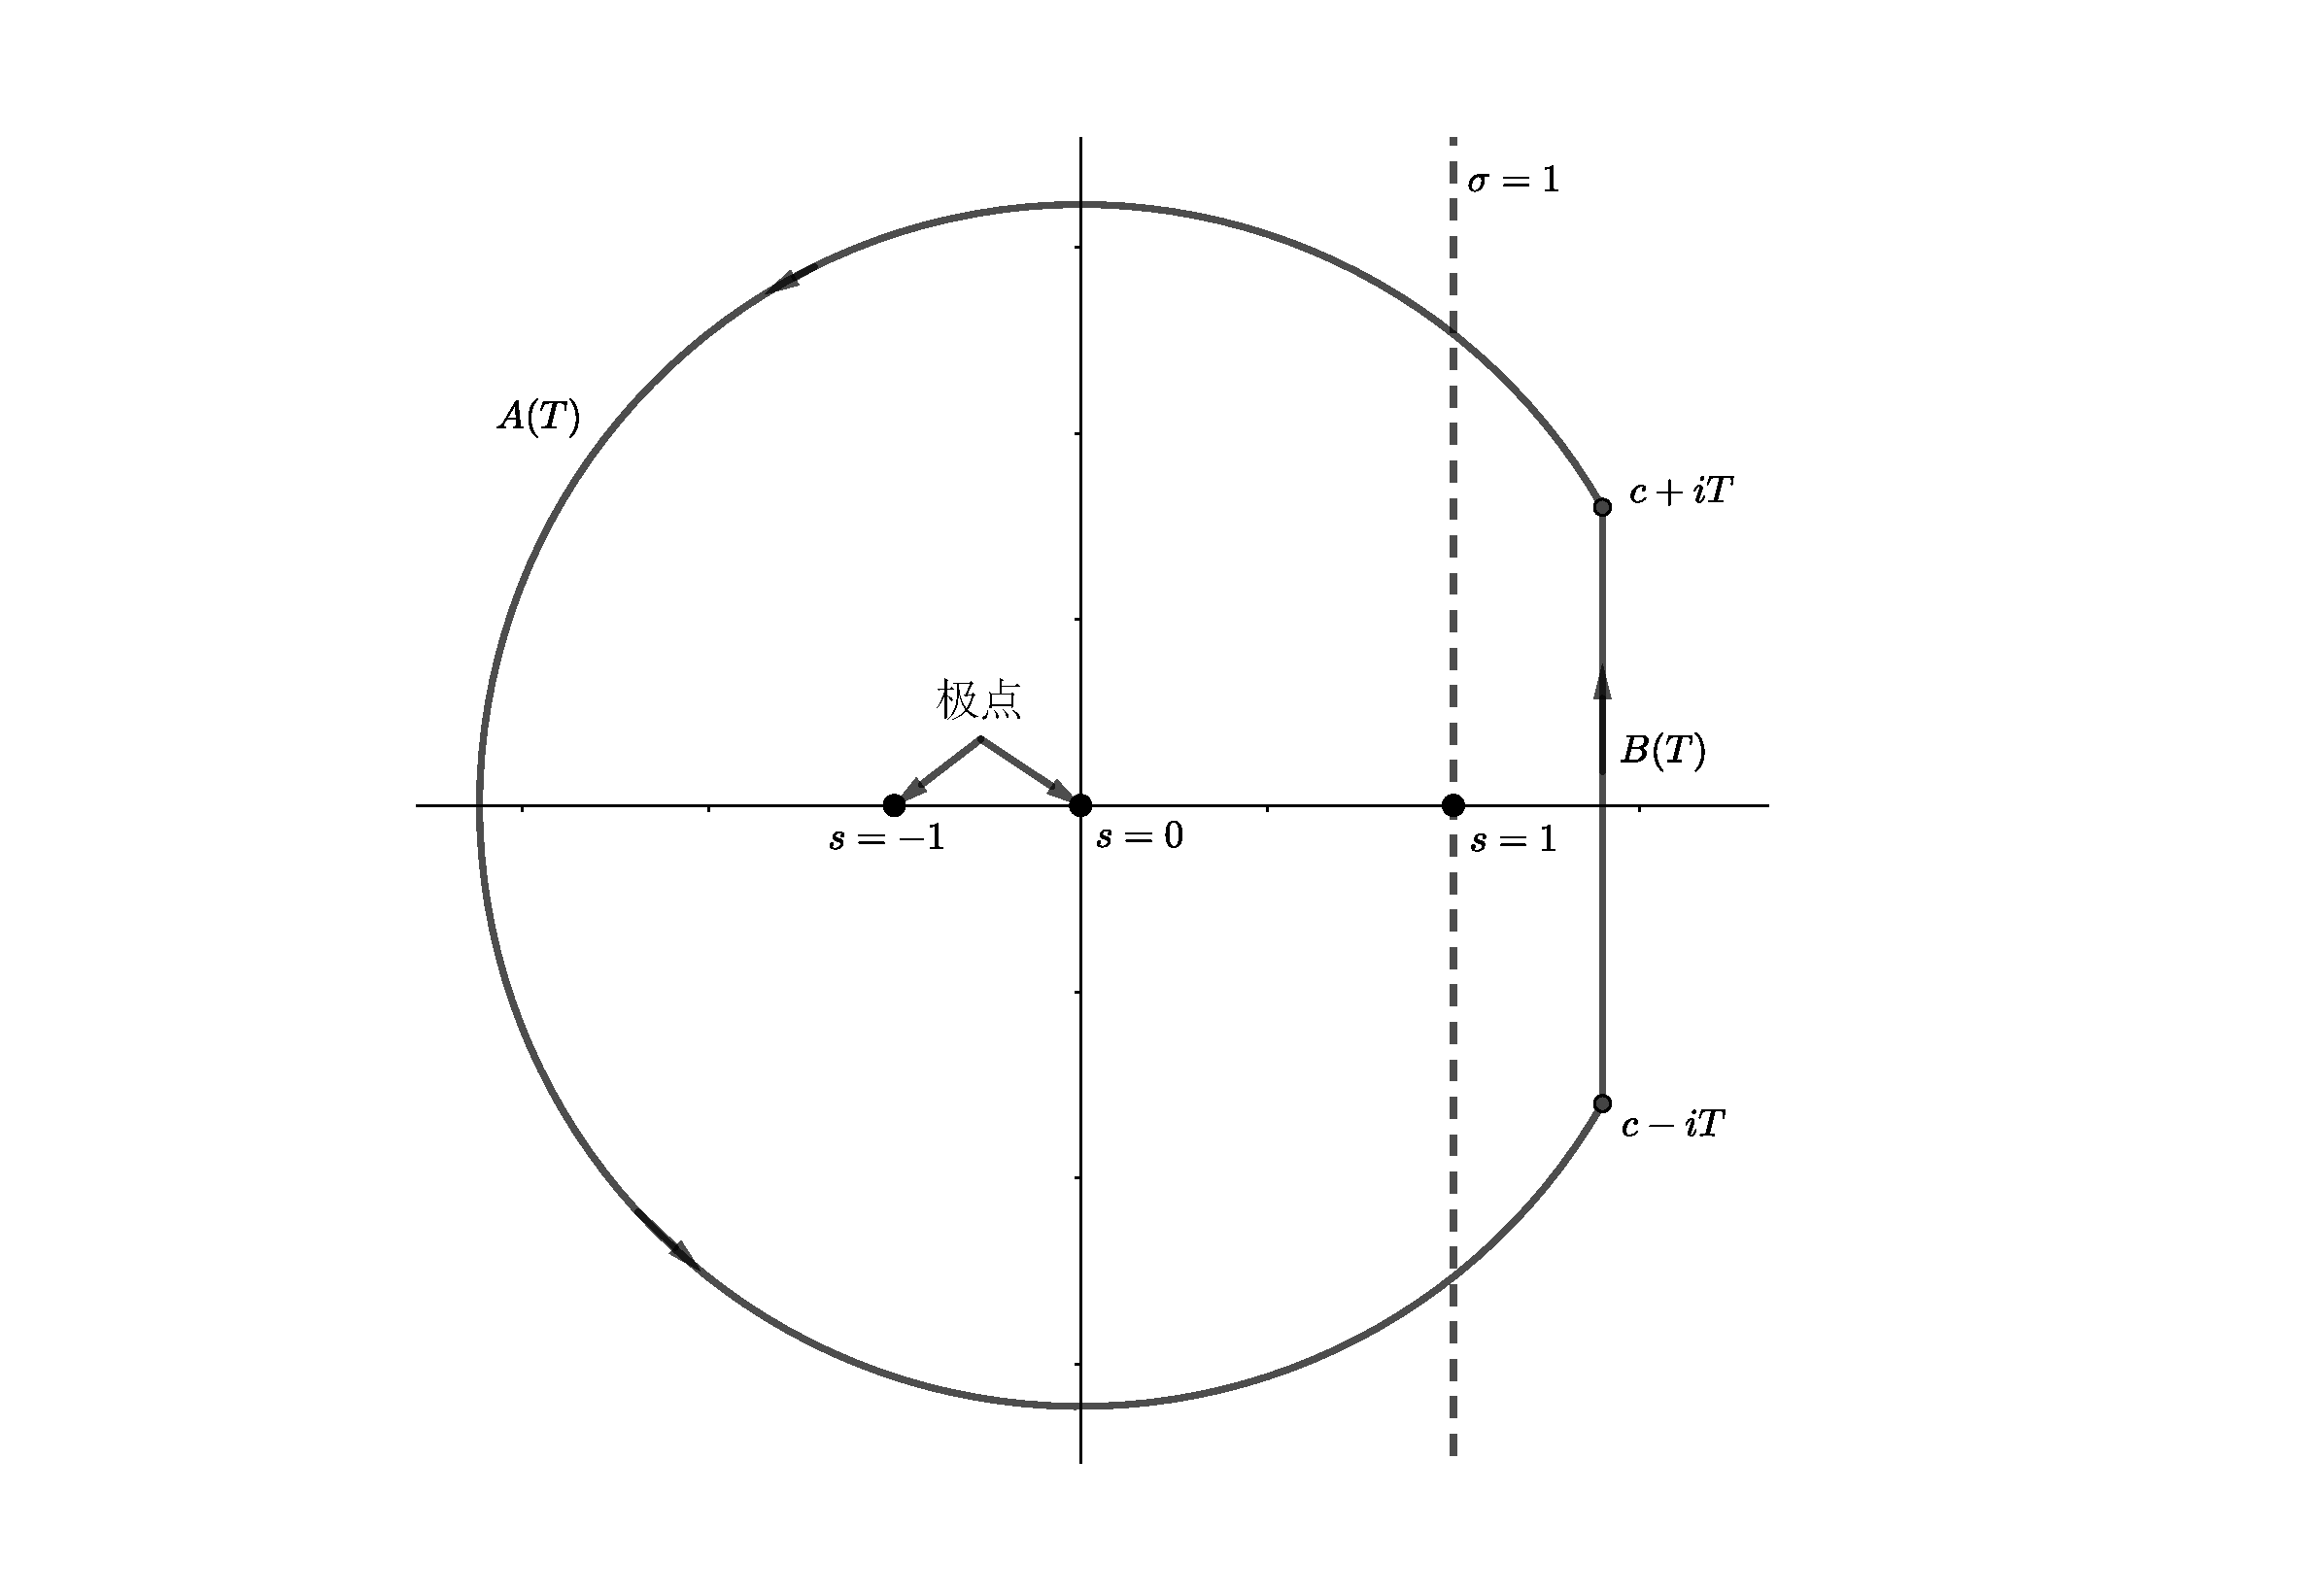
\includegraphics[scale=0.5]{引理计算psi1_1.pdf}
        \caption{$a\geq 1$时构造的曲线}
        \label{figure-psi1}
    \end{figure}

    由留数定理知
    \begin{equation}\label{eq-psi1}
        \begin{aligned}
            \frac{1}{2\pi \i}\int_{\gamma(T)}\frac{a^s}{s(s+1)}\,\d s =&\ \frac{1}{2\pi \i}\int_{A(T)}f(s)\,\d s+\frac{1}{2\pi\i}\int_{B(T)}f(s)\,\d s\\
            =&\ \res(f, 0)+\res(f, -1) = 1 - \frac{1}{a},
        \end{aligned}
    \end{equation}
    下面证明当$T\to\infty$时, $\frac{1}{2\pi \i}\int_{A(T)}f(s)\,\d s=0$.\add

    设$s\in A(T)$, 记$R = \sqrt{c^2+T^2} = |s|$, 由于$a\geq 1$且$\sigma \leq c$, 则$|a^s| = a^{\sigma}\leq a^c$, 于是
    \begin{equation}\label{eq-psi0}
        \begin{aligned}
            \left|\frac{1}{2\pi\i}\int_{A(T)}\frac{a^s}{s(s+1)}\,\d s\right|\leq&\ \frac{1}{2\pi}\int_{A(T)}\frac{|a^s|}{|s||s+1|}\,|\d s|\\
            \leq&\ \frac{1}{2\pi}\,\frac{a^c}{R(R-1)}\cdot 2 \pi R = \frac{a^c}{R-1}\leq \frac{a^c}{T-1}\to 0\quad(T\to \infty).
        \end{aligned}
    \end{equation}

    所以, 当$T\to\infty$时, 由(\ref{eq-psi1})式可知
    \begin{equation*}
        \lim_{T\to\infty}\frac{1}{2\pi\i}\int_{B(T)}f(s)\,\d s=\lim_{T\to \infty}\frac{1}{2\pi\i}\int_{c-\i T}^{c+\i T}\frac{a^s}{s(s+1)}\,\d s=\frac{1}{2\pi \i}\int_{c-\i\infty}^{c+\i\infty}\frac{a^s}{s(s+1)}\,\d s = 1-\frac{1}{a}.
    \end{equation*}

    当$0 < a < 1$时, 类似地, 构造圆弧$C(T) = \{z:|z|\leq \sqrt{c^2+T^2},\sigma > c\}$, 设$\Gamma(T) = B^-(T)\cup C(T)$定向为逆时针方向, 其中$B^-(T)$的定向与$B(T)$的定向相反. 如\textbf{图}\ref{figure-psi2}所示.
    \begin{figure}[htbp] % h: 当前位置, t: 顶部, b: 底部, p: 浮动页, 这样组合指的是使用这个顺序进行排版
        \centering
        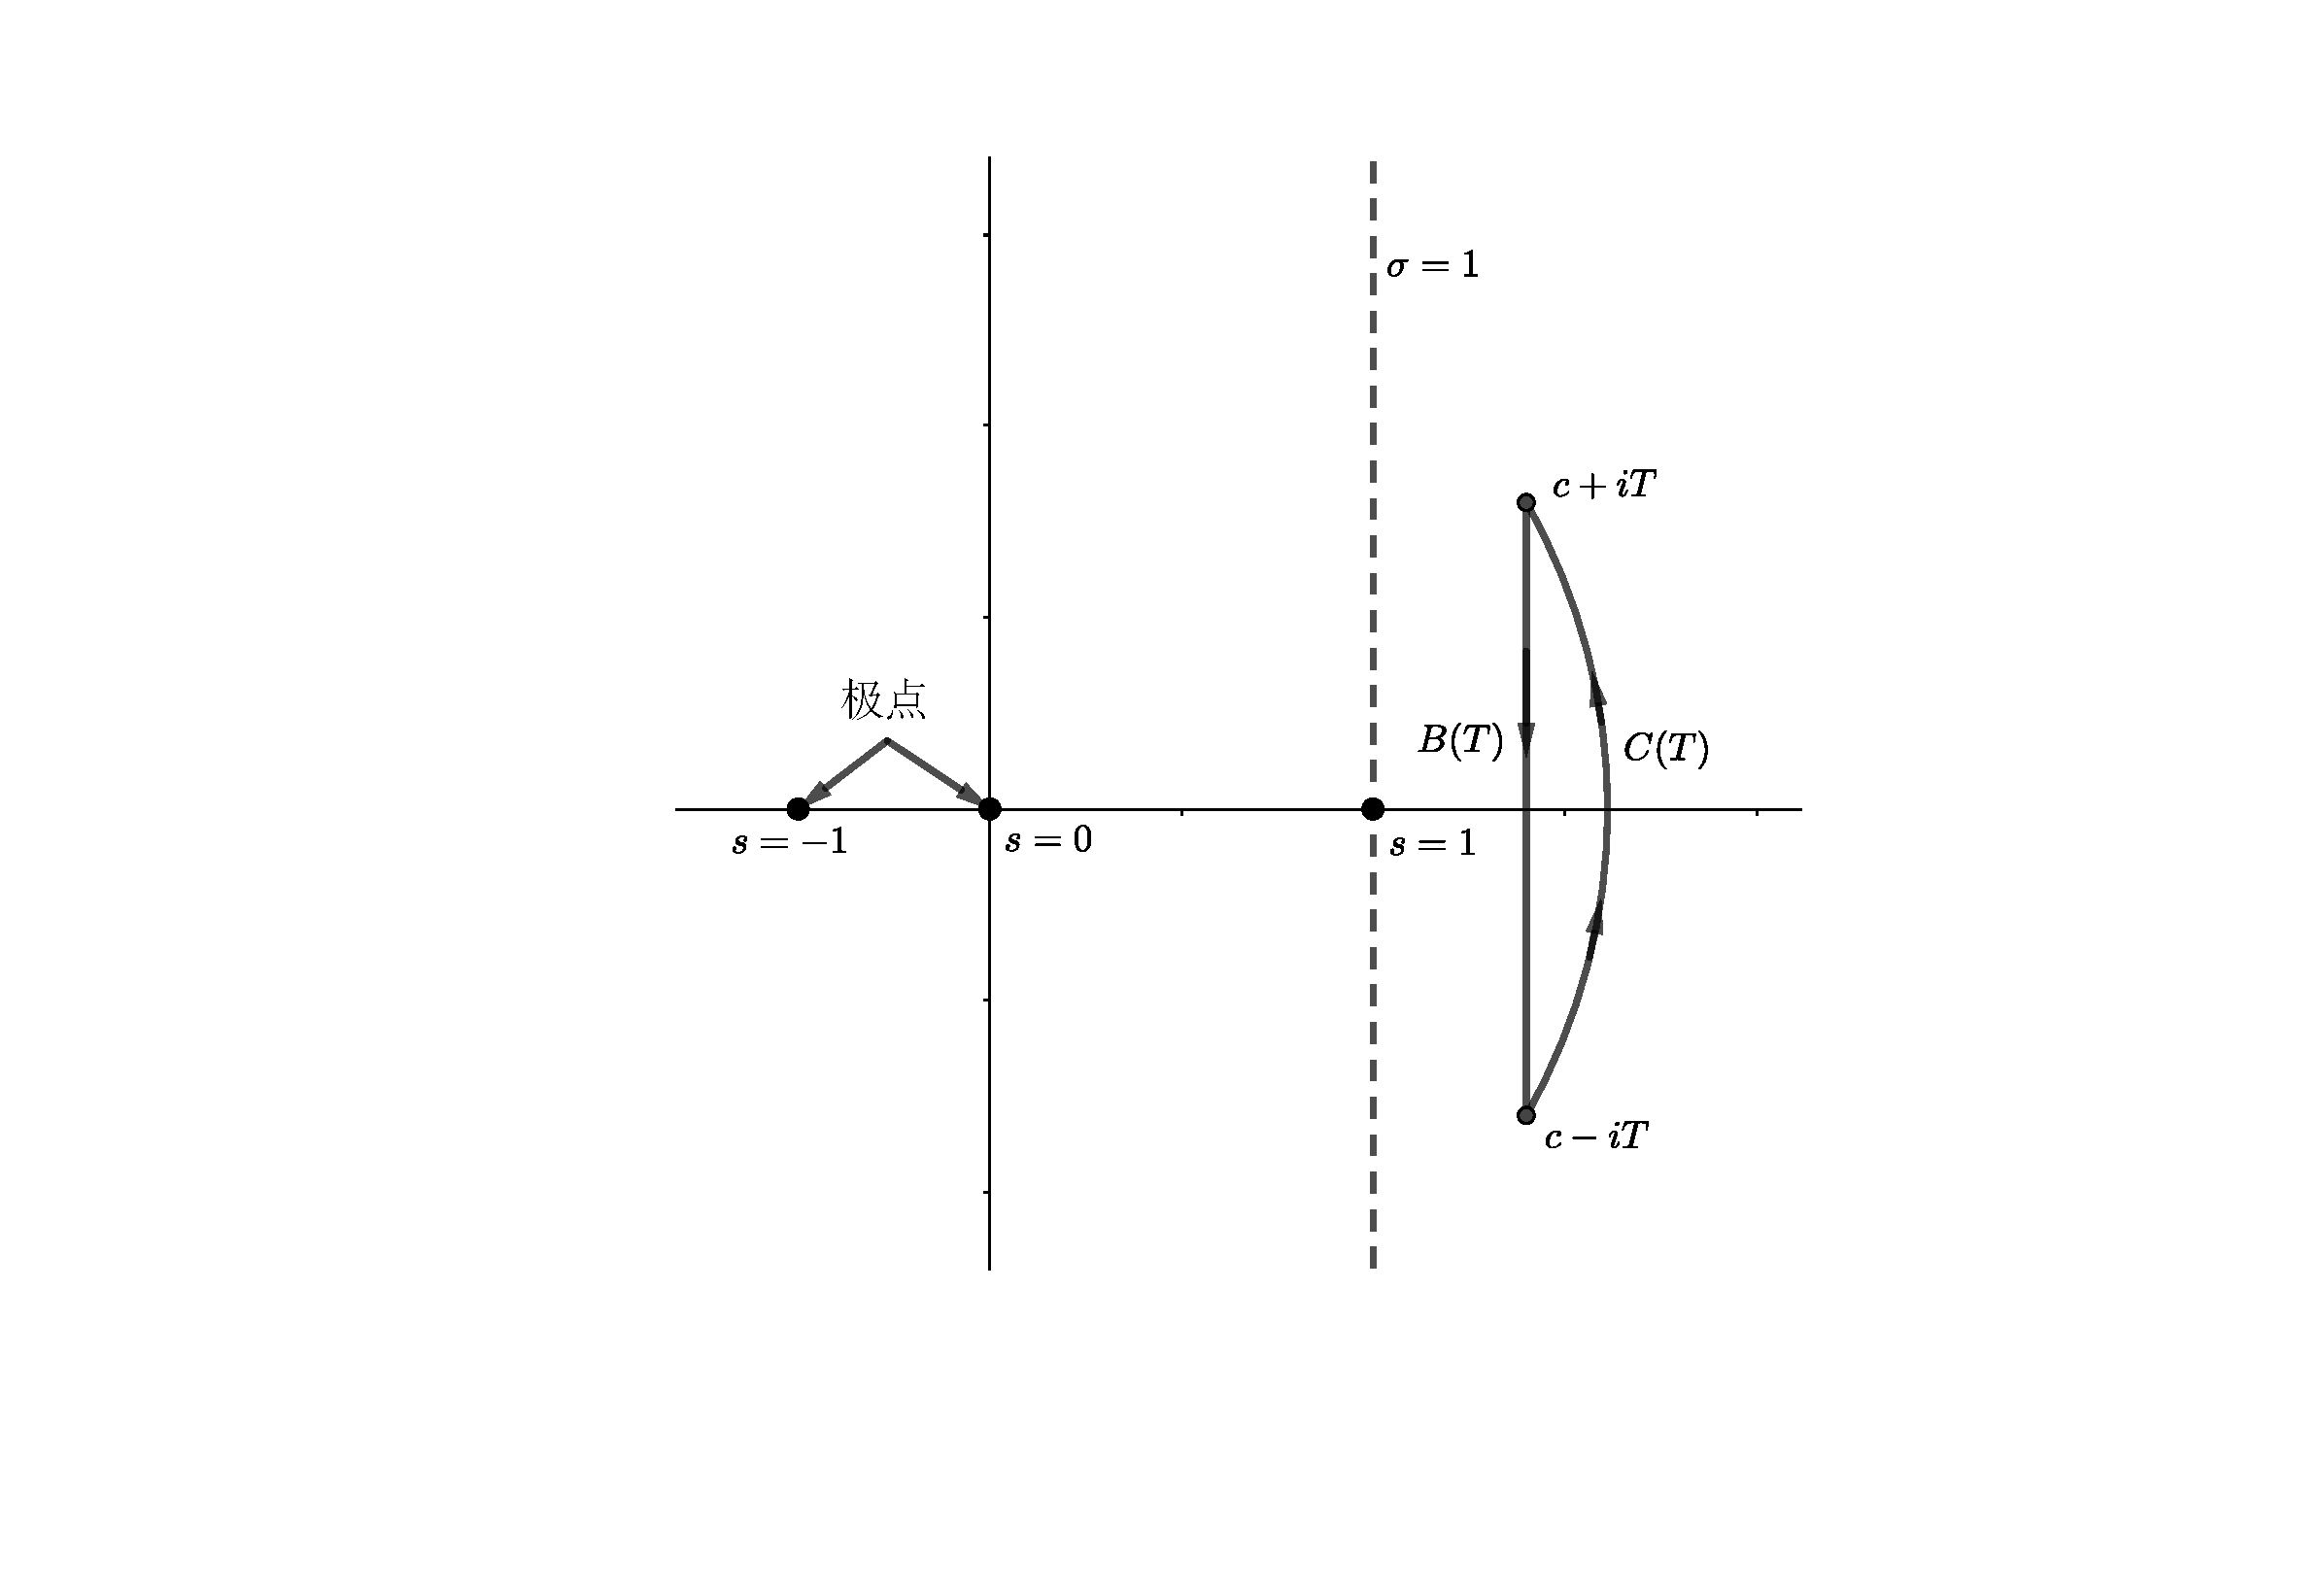
\includegraphics[scale=0.5]{引理计算psi1_2.pdf}
        \caption{$0 < a < 1$时构造的曲线}
        \label{figure-psi2}
    \end{figure}
    
    由于$f(s)$在$\Gamma(T)$所围成的区域中解析, 由Cauchy定理知
    \begin{equation}\label{eq-psi2}
        0=\int_{\Gamma(T)}f(s)\,\d s=\int_{C(T)}f(s)\,\d s +\int_{B^-(T)}f(s)\,\d s=\int_{C(T)}f(s)\,\d s-\int_{B(T)}f(s)\,\d s
    \end{equation}
    由于当$s\in C(T)$时, $0 < a < 1$且$\sigma \geq c$, 则$|a^s|=a^\sigma\leq a^c$, \add 类似(\ref{eq-psi0})式, 可以证明$\frac{1}{2\pi\i}\int_{C(T)}f(s)\,\d s = 0$.

    所以当$T\to \infty$时, 由(\ref{eq-psi2})式可知
    \begin{equation*}
        \lim_{T\to\infty}\int_{B(T)}f(s)\,\d s = \frac{1}{2\pi\i}\int_{c-\i\infty}^{c+\i\infty}\frac{a^s}{s(s+1)}\,\d s = 0.
    \end{equation*}
\end{proof}
\begin{proposition}\label{prop-psi-zeta}
    设$x>0$, $c > 1$, 则
    \begin{equation*}
        \psi_1(x) = \frac{1}{2\pi\i}\int_{c-\i\infty}^{c+\i\infty}\frac{x^{s+1}}{s(s+1)}\left(-\frac{\zeta'(s)}{\zeta(s)}\right)\,\d s,
    \end{equation*}
    其中积分路线为直线$\sigma = c$.
\end{proposition}
\begin{proof}
    由\textbf{引理}\ref{le-psi}, \textbf{命题}\ref{prop-zeta-lambda}和\textbf{命题}\ref{prop-psi-lambda}可得
    \begin{equation*}
        \begin{aligned}
            \frac{1}{2\pi\i}\int_{c-\i\infty}^{c+\i\infty}\frac{x^{s+1}}{s(s+1)}\left(-\frac{\zeta'(s)}{\zeta(s)}\right) \xlongequal{\textbf{命题}\ref{prop-zeta-lambda}}&\  \frac{1}{2\pi\i}\int_{c-\i\infty}^{c+\i\infty}\frac{x^{s+1}}{s(s+1)}\sum_{n=1}^\infty\frac{\Lambda(n)}{n^s}\,\d s\\
            =&\ x\sum_{n=1}^\infty\Lambda(n)\frac{1}{2\pi\i}\int_{c-\i\infty}^{c+\i\infty}\frac{(x/n)^s}{s(s+1)}\,\d s\\
            \xlongequal{\textbf{引理}\ref{le-psi}}&\ x\sum_{n=1}^\infty\Lambda(n)\left(1-\frac{n}{x}\right)\\
            \xlongequal{\textbf{命题}\ref{prop-psi-lambda}}&\ \sum_{n=1}^\infty\Lambda(n)(x-n)=\psi_1(x).
        \end{aligned}
    \end{equation*}
\end{proof}
这样我们就找到了$\psi_1(x)$的复积分形式, 并且积分中含有$\zeta(s)$函数, 进一步得到素数定理的另一充分条件, 也就是我们最终所要证明的. 
\begin{proposition}\label{prop-goto-int}
    设$G(s) = \frac{1}{s(s+1)}\left(-\frac{\zeta'(s)}{\zeta(s)}\right)$, 当$x\to\infty$时, 若
    \begin{equation}\label{eq-goto-int}
        \frac{1}{2\pi\i}\int_{c-\i\infty}^{c+\i\infty}G(s)x^{s-1}\,\d s\sim\frac{1}{2}
    \end{equation}
    成立, 则素数定理成立.
\end{proposition}
\begin{proof}
    由第二节\textbf{命题}\ref{prop-goto-psi1}知, $\psi_1(x)\sim\frac{1}{2}x^2$是素数定理的充要条件, 根据\textbf{命题}\ref{prop-psi-zeta}得
    \begin{equation*}
        \frac{\psi_1(x)}{x^2} = \frac{1}{2\pi\i}\int_{c-\i\infty}^{c+\i\infty}\frac{x^{s-1}}{s(s+1)}\left(-\frac{\zeta'(s)}{\zeta(s)}\right)\,\d s = \frac{1}{2\pi\i}\int_{c-\i\infty}^{c+\i\infty}G(s)x^{s-1}\,\d s,
    \end{equation*}

    所以(\ref{eq-goto-int})式成立, 则素数定理成立.
\end{proof}
由于$\zeta(s),\ \zeta'(s)$在半平面$\sigma>1$上解析, 且$\zeta(s)$不为$0$, 所以$G(s)$在半平面$\sigma > 1$上解析. 我们期望利用留数定理计算$G(s)x^{s-1}$在直线$\sigma =c$上的积分, 发现$\zeta(s)$在$s=1$处发散, 那么可不可以将$\zeta(s)$延拓到半平面$\sigma > 0$上, 且$s=1$为$\zeta(s)$的唯一极点, 也就是说将$\zeta(s)$延拓为半平面$\sigma>0$上的亚纯函数, 于是$G(s)$是否也是$\sigma > 0$上的亚纯函数, 有唯一的极点$s=1$. 于是, 我们就可以利用$s=1$处留数计算$G(s)x^{s-1}$在直线$\sigma = c$上的积分了. 所以, 接下来我们将对$\zeta(s)$进行解析延拓.
\section{zeta函数的解析延拓}
\begin{definition}[解析延拓]
    设函数$f(s)$为定义在开集$D$上的解析函数, 若存在定义在开集$U$上的解析函数$F(s)$, 其中$D\subset U$, 对任意$s\in D$有$f(s) = F(s)$成立, 则称函数$F(s)$为函数$f(s)$的解析延拓.
\end{definition}
因此解析延拓就是将一个解析函数延拓到解析域外, 并且使得该函数在更大的区域上保持解析性质. 下面考虑将$\zeta(s)$解析延拓到半平面$\sigma > 0$去掉奇点$s=1$, 即在集合$D := \{s\in \C:\sigma > 0, s\neq 1\}$上解析.
\begin{lemma}\label{le-int1}
    设可积函数$f:\R\to\C$, 则
    \begin{equation*}
        \sum_{n=1}^m\int_n^{m+1}f(x)\,\d x=\sum_{n=1}^mn\int_n^{n+1}f(x)\,\d x.
    \end{equation*}
    \begin{proof}设函数$g_n(k) = \begin{cases}
        0,&\quad k < n,\\
        1,&\quad k \geq n.
    \end{cases}$, 则
        \begin{equation*}
            \begin{aligned}
                \sum_{n=1}^m\int_n^{m+1}f(x)\,\d x =&\ \sum_{n=1}^m\sum_{k=n}^m\int_{k}^{k+1}f(x)\,\d x = \sum_{n=1}^m\sum_{k=1}^m\int_{k}^{k+1}f(x)\,\d xg_n(k)\\
                =&\ \sum_{k=1}^m\int_{k}^{k+1}f(x)\,\d x\sum_{n=1}^mg_n(k) = \sum_{k=1}^m\int_k^{k+1}f(x)\,\d x\sum_{n=1}^k1\\
                =&\ \sum_{k=1}^mk\int_{k}^{k+1}f(x)\,\d x.
            \end{aligned}
        \end{equation*}
    \end{proof}
\end{lemma}
上述定理表明整数的积分区间, 可以分为多个长度为$1$的积分累积.
\begin{lemma}\label{le-int2}
    对定义域为$\R$的函数$f(x)$, 任意$x > 1$, 有
    \begin{equation*}
        \sum_{n\leq x}\int_n^xf(u)\,\d u = \int_1^x[u]f(u)\,\d u.
    \end{equation*}
\end{lemma}
\begin{proof}
    \begin{equation*}
        \begin{aligned}
            \sum_{n\leq x}\int_n^xf(u)\,\d u=&\ \sum_{n=1}^{[x]-1}\int_n^{[x]}f(u)\,\d u + \sum_{n=1}^{[x]}\int_{[x]}^xf(u)\,\d u\\
            \xlongequal{\textbf{引理}\ref{le-int1}}&\ \sum_{n=1}^{[x]-1}n\int_n^{n+1}f(u)\,\d u+[x]\int_{[x]}^xf(u)\,\d u\\
            =&\ \sum_{n=1}^{[x] - 1}\int_n^{n+1}[u]f(u)\,\d u+\int_{[x]}^x[u]f(u)\,\d u\\
            =&\ \int_1^x[u]f(u)\,\d u.
        \end{aligned}
    \end{equation*}
\end{proof}
\begin{lemma}\label{le-int3}
    设$D$为$\C$中的开集, $\gamma$为$\C$中可求长曲线, 函数$f(s, t):D\times \gamma\to \C$, 对任意$s\in D$, $f(s, t)$在$\gamma$上连续, 任意$t\in \gamma$, $f(s, t)$在$D$内解析, 则$F(s) = \int_{\gamma}f(s, t)\,\d t$在$D$内解析.
\end{lemma}
\begin{proof}
    由于$f(s, t)$在$\gamma$上连续, 则$F(s)$有意义. 设$\Gamma$为$D$内任一可求长简单闭曲线, 其所围成的区域包含于$D$, 由Fubini定理知
    \begin{equation*}
        \int_{\Gamma}F(s)\,\d s=\int_{\Gamma}\,\d s\int_{\gamma}f(s, t)\,\d t = \int_{\gamma}\,\d t\int_{\Gamma}f(s, t)\,\d s.
    \end{equation*}
    根据Cauchy定理$\int_{\Gamma}f(s, t)\,\d s = 0$, 则$\int_{\Gamma}F(s)\,\d s = 0$, 由Morera定理知, $F(z)$在$D$内解析.
\end{proof}
\begin{theorem}\label{thm-zeta}
    $\zeta(s)$存在$D=\{s:\sigma > 0, s\neq 1\}$上的解析延拓, 且有唯一的一级极点$s = 1$.
\end{theorem}
\begin{proof}
    先考虑$\zeta(s)$的部分和, 对任意$x \geq 1$有
    \begin{equation*}
        \sum_{n\leq x}\frac{1}{n^s}-\sum_{n\leq x}\frac{1}{x^s} = \sum_{n\leq x}\int_n^x\frac{s}{u^{s+1}}\,\d u
        \xlongequal{\textbf{引理}\ref{le-int2}} s\int_1^x\frac{[u]}{u^{s+1}}\,\d u
    \end{equation*}
    则
    \begin{equation}\label{eq-zeta-sub}
        \begin{aligned}
            \sum_{n\leq x}\frac{1}{n^s} =&\ \frac{[x]}{x^s}+s\int_1^x\frac{[u]}{u^{s+1}}\,\d u = \frac{x-\{x\}}{x^s}+s\int_1^x\frac{1}{u^s}\,\d u-s\int_1^x\frac{\{u\}}{u^{s+1}}\,\d u\\
            =&\ \frac{1}{x^{s-1}}-\frac{\{x\}}{x^s}+\frac{s}{s-1}-\frac{s}{(s-1)x^{s-1}}-s\int_1^x\frac{\{u\}}{u^{s+1}}\,\d u
        \end{aligned}
    \end{equation}
    对于$\sigma >1$时
    \begin{equation*}
        \zeta(s) = \lim_{x\to\infty}\sum_{n\leq x}\frac{1}{n^s}=\frac{s}{s-1}-s\int_1^{\infty}\frac{\{u\}}{u^{s+1}}\,\d u.
    \end{equation*}

    定义函数
    \begin{equation}\label{eq-zeta-ex}
        g(s) = \begin{cases}
            \frac{s}{s-1}-s\int_1^{\infty}\frac{\{u\}}{u^{s+1}}\,\d u,&\quad s\in D,\\
            0,&\quad s\neq 1.
        \end{cases}
    \end{equation}
    下面证明$\int_1^{\infty}\frac{\{u\}}{u^{s+1}}\,\d u$在$D$上是解析的. 设$F_n(u) = \int_n^{n+1}\frac{\{u\}}{u^{s+1}}\,\d u$, 则
    \begin{equation*}
    \int_1^{\infty}\frac{\{u\}}{u^{s+1}} = \sum_{n=1}^\infty F_n(u).
    \end{equation*}

    注意到
    \begin{equation*}
        F_n(s) = \int_0^1\frac{\{n+t\}}{(n+t)^{s+1}}\,\d t=\int_0^1\frac{t}{(n+t)^{s+1}}\,\d t.
    \end{equation*}
    由\textbf{引理}\ref{le-int3}可得$F_n(s)$在$D$上解析.

    对任意$\epsilon > 0$, 取$\sigma > \sigma$, 则
    \begin{equation*}
        |F_n(s)|\leq \int_n^{n+1}\left|\frac{\{u\}}{u^{s+1}}\right|\,\d u\leq \int_n^{n+1}\frac{1}{|u^{s+1}|}\,\d u=\int_n^{n+1}\frac{1}{u^{\sigma+1}}\,\d u\leq \frac{1}{n^{\sigma + 1}}\leq \frac{1}{n^{\epsilon+1}}.
    \end{equation*}

    由于级数$\sum_{n=1}^\infty\frac{1}{n^{\epsilon + 1}}$收敛, 由M-判别法知, 级数$F_n(s)$一致收敛到$\int_1^{\infty}\frac{\{u\}}{u^{s+1}}\,\d u$, \\由 \nameref{thm-weierstrass} 定理知$\int_1^{\infty}\frac{\{u\}}{u^{s+1}}\,\d u$在$D$上解析.

    设$A(s) = s-s(s-1)\int_1^{\infty}\frac{\{u\}}{u^{s+1}}\,\d u,\ B(s) = s-1$, 则
    \begin{equation*}
    g(s) = \frac{A(s)}{B(s)}\quad(s\neq 1),
    \end{equation*}
    由于$P(1) = 1,\ Q(1) = 0,\ Q'(1) = 1$, 所以$s=1$是$g(s)$的一级极点.

    综上, $g(s)$是$\zeta(s)$在$D$上的解析延拓且$s=1$是$g(s)$的一级极点.
\end{proof}
\section{G(s)的上界估计, zeta的零点}
根据\textbf{命题}\ref{prop-goto-int}可知, 我们需要对$\frac{1}{2\pi\i}\int_{c-\i \infty}^{c+\i \infty}G(s)x^{s-1}\,\d s$使用留数定理计算,\\ 其中$G(s) = \frac{1}{s(s+1)}\left(-\frac{\zeta'(s)}{\zeta(s)}\right)$\add. 因此我们可能需要$G(x)$的上界估计, \textbf{定理}\ref{thm-zeta}我们通过解析延拓得到了$\zeta(s)$函数在半平面$\sigma > 0$除$s=1$上解析, 则$G(s)$在半平面$\sigma > 0$除$s=1$和$\zeta(s)$的零点外解析, 由\textbf{命题}\ref{prop-zeta-zero1}知, $\zeta(s)$在半平面$\sigma > 1$上无零点, 所以$G(x)$在$\sigma > 1$上解析, 我们期望$G(x)$在半平面$\sigma \geq 1$上是亚纯函数且有唯一极点$s=1$, 这样才能使用留数定理计算积分.

所以接下来, 我们将估计$G(x)$的上界并证明$\zeta(s)$在直线$\sigma =1$上无零点.

%\begin{definition}[孤立零点]
%    若$z_0$为$f(z)$的零点, 存在去心邻域$V^*(z_0;\delta) = \{z\in\C: 0 < |z-z_0|< \delta\}$, 使得$f(z)$在$V^*(z_0;\delta)$内不含零点, 则称$z_0$为$f(z)$的孤立零点.
%\end{definition}
%\begin{theorem}
%    函数$f(z)$在区域$D$内解析且不恒为零, 则$f(z)$在$D$内的零点是孤立的.
%\end{theorem}
%上述定理证明请见\cite{ref-复变函数}第五章定理10, 该定理说明, 若函数$f(z)$在一个闭区域$\bar{\Omega}$上解析, 则$f(z)$在$\Omega$上只能有有限个零点, 否则, 零点序列在$\bar{\Omega}$上就存在极限点$z_0$且$f(z_0) = 0$, 而$z_0$不是孤立零点, 与零点独立性矛盾.
%
%所以, 我们可以在有界区域中挖去有限个零点, 从而使得$\zeta(s)$在该区域中无零点, 于是$G(x)$在该区域上解析.

\begin{theorem}[Cauchy公式]
    设区域$D$是可求长简单闭曲线$\gamma$所围成的内部, 函数$f(z)$在$D$内解析, $\bar{D}$上连续, 对任意$z\in D$有
    \begin{equation*}
        f^{(n)}(z) = \frac{n!}{1\pi\i}\int_{\gamma}\frac{f(\xi)}{(\xi-z)^{n+1}}\,\d \xi\quad(n=0,1,2,\cdots).
    \end{equation*}
\end{theorem}
证明请见\cite{ref-复变函数}第四章定理4.
\begin{lemma}\label{lemma-upper}
    设$s\in\C$, $s= \sigma + \i t$, $\sigma \geq 1$, $t\geq 2$, 则

    (1) $\zeta(s) = O(\log t)$,

    (2) $\zeta'(s) = O(\log^2 t)$,

    (3) 设$\delta\in(0,1)$, 若$\sigma \geq \delta$且$t\geq 1$, 则$\zeta(s) = O_{\delta}(t^{1-\delta})$, 即$|\zeta(s)|\leq Ct^{1-\delta}$, 其中$C_{\delta}$与$\delta$相关.
\end{lemma}
\begin{proof}
    由\textbf{定理}\ref{thm-zeta}中(\ref{eq-zeta-sub})和(\ref{eq-zeta-ex})式可知, 当$\sigma > 0, t\geq 1, s\neq 1$, 对任意$x \geq 1$有
    \begin{equation*}
        \zeta(s)=\frac{s}{s-1}-s\int_1^{\infty}\frac{\{u\}}{u^{s+1}}\,\d u,\quad\sum_{n\leq x}\frac{1}{n^s}=\frac{1}{x^{s-1}}-\frac{\{x\}}{x^s}+\frac{s}{s-1}-\frac{s}{(s-1)x^{s-1}}-s\int_1^x\frac{\{u\}}{u^{s+1}}\,\d u,
    \end{equation*}
    则
    \begin{equation}\label{eq-upper1}
        \zeta(s)-\sum_{n\leq x}\frac{1}{n^s}= \frac{\{x\}}{x^s}+\frac{1}{(s-1)x^{s-1}}-s\int_1^x\frac{\{u\}}{u^{s+1}}\,\d u,
    \end{equation}
    注意到
    \begin{equation*}
        \begin{aligned}
            &\ \left|\sum_{n\leq x}\frac{1}{n^s}\right|\leq \sum_{n\leq x}\frac{1}{x^{\sigma}},\qquad \left|\frac{\{x\}}{x^s}\right|\leq \frac{1}{x^\sigma},\qquad\left|\frac{1}{(s-1)x^{s-1}}\right|\leq\frac{1}{tx^{\sigma -1}}\leq \frac{1}{x^{\sigma -1}},\\
            &\ \left|s\int_x^{\infty}\frac{\{u\}}{u^{s+1}}\,\d u\right|\leq \sqrt{\sigma^2+t^2}\int_x^{\infty}\frac{1}{u^{\sigma +1}}\,\d u\leq \frac{\sigma + t}{\sigma x^\sigma} = \left(1+\frac{t}{\sigma}\right)\frac{1}{x^{\sigma}},
        \end{aligned}
    \end{equation*}
    由(\ref{eq-upper1})式知
    \begin{equation}\label{eq-upper2}
        |\zeta(s)|\leq \left|\sum_{n\leq x}\frac{1}{n^s}\right|+\left|\frac{\{x\}}{x^{s-1}}\right|+\left|\frac{1}{(s-1)x^{s-1}}\right|+\left|s\int_x^{\infty}\frac{\{u\}}{u^{s+1}}\,\d u\right|\leq \sum_{n\leq x}\frac{1}{n^{\sigma}}+\frac{1}{x^{\sigma - 1}}+\left(2+\frac{t}{\sigma}\right)\frac{1}{x^\sigma}.
    \end{equation}
    若$\sigma\geq 1$, 则
    \begin{equation*}
        \begin{aligned}
            &\ |\zeta(s)|\leq\sum_{n\leq x}\frac{1}{n}+1+\frac{2+t}{x}\leq \sum_{n=1}^{[x]-1}\int_n^{n+1}\frac{1}{n}\,\d u+2+\frac{2+t}{x}\\
            &\ \leq \int_1^x\frac{1}{u}\,\d u+4+\frac{t}{x} = \log x+4+\frac{t}{x},
        \end{aligned}
    \end{equation*}
    取$x= t$, 得
    \begin{equation}\label{eq-upper3}
        |\zeta(s)|\leq \log t+5.
    \end{equation}
    于是(1)得证.

    任意$\delta\in (0,1)$, 若$\sigma > \delta$, 由(\ref{eq-upper2})式得
    \begin{equation*}
        |\zeta(s)|\leq \sum_{n\leq x}\frac{1}{n^{\delta}}+\frac{1}{x^{\delta-1}}+\left(2+\frac{t}{\delta}\right)\frac{1}{x^{\delta}},
    \end{equation*}
    由于
    \begin{equation*}
        \sum_{n\leq x}\frac{1}{n^{\delta}} = \sum_{n=1}^{[x]}\frac{1}{n^{\delta}}\leq \sum_{n=1}^{[x]-1}\int_{n-1}^n\frac{\,\d x}{x^{\delta}}\leq \int_0^x\frac{\,\d x}{x^{\delta}}\leq \frac{x^{1-\delta}}{1-\delta}
    \end{equation*}
    则
    \begin{equation*}
        |\zeta(s)|\leq \frac{x^{1-\delta}}{1-\delta}+x^{1-\delta}+\frac{3t}{\delta x^{\delta}},
    \end{equation*}
    取$x=t$, 得
    \begin{equation}\label{eq-upper4}
        |\zeta(s)|\leq t^{1-\delta}\left(\frac{1}{1-\delta}+1+\frac{3}{\delta}\right).
    \end{equation}
    于是(3)得证.

    任取一点$s_0 = \sigma_0+\i t_0$, $\sigma_0\geq 1,\ t_0\geq 2$, 设$D = V(s_0;\rho)$\add, 即以$s_0$为圆心半径为$\rho$的圆围成的区域, 其中$0 < \rho < \frac{1}{2}$, $\gamma$为$D$的边界, 则$\zeta(s)$在$\gamma$内解析.

    于是
    \begin{equation*}
        |\zeta'(s_0)|=\left|\frac{1}{2\pi\i}\int_{\gamma}\frac{\zeta(\xi)}{(\xi-s_0)^2}\,\d\xi\right|\leq\frac{M}{\rho},
    \end{equation*}
    其中$M = \sup_{s\in D}\xi(s)$, 下面对$M$进行估计.

    对于$s\in D$, 有$\sigma > \sigma_0 - \rho\geq 1-\rho > 0$, 取$\delta = 1-\rho$, 由(\ref{eq-upper4})式得
    \begin{equation*}
        |\zeta(s)|\leq t^{\rho}\left(\frac{1}{\rho}+1+\frac{3}{1-\rho}\right),
    \end{equation*}
    由于$0<\rho < \frac{1}{2}$且$1\leq t_0-\rho < t < t_0+\rho < 2t_0$, 于是
    \begin{equation*}
        |\zeta(s)|\leq (2t_0)^{\rho}\left(\frac{1}{\rho}+\frac{1}{\rho}+\frac{3}{\rho}\right)\leq\frac{10t_0^{\rho}}{\rho},
    \end{equation*}
    则
    \begin{equation*}
        |\zeta'(s)|\leq \frac{10t_0^{\rho}}{\rho^2},
    \end{equation*}
    取$\rho = \frac{1}{\log t_0 + 2}$, 则$\rho < \frac{1}{\log t_0}$, $t_0^{\rho} = e^{\rho\log t_0} < e$, 所以$|\zeta'(s_0)|\leq 10e(\log t_0+2)^2$, 于是(2)得证.
\end{proof}
\begin{proposition}\label{prop-zero-upper}
    $\zeta(s)$在直线$\sigma = 1$上没有零点, 当$\sigma \geq 1$时, 有
    \begin{equation*}
        \frac{1}{\zeta(s)} = O(\log^7 t)\quad(t\to\infty).
    \end{equation*}
\end{proposition}
\begin{proof}
    由于$\zeta(s) = \prod_p\frac{1}{1-p^{-s}}$, 则
    \begin{equation*}
        \log \zeta(s) = \prod_p\log\frac{1}{1-p^{-s}}
    \end{equation*}
    设$x = p^{-s}$, 则$x < 1$, 注意到
    \begin{equation*}
        \log\frac{1}{1-x}=\int_0^x\frac{1}{1-u}\,\d u = \int_0^x\sum_{m=0}^\infty u^m\,\d u=\sum_{m=0}^\infty\int_0^x u^m\,\d u = \sum_{m=0}^\infty\frac{x^{m+1}}{m+1} = \sum_{m=1}^\infty\frac{x^m}{m},
    \end{equation*}
    所以
    \begin{equation*}
        \log\zeta(s) = \sum_{p}\sum_{m=1}^\infty\frac{(p^m)^{-s}}{m} = \sum_{p}\sum_{n=p^m}\frac{n^{-s}}{m}
    \end{equation*}
    令$c_n = \begin{cases}
        \frac{1}{m},&\quad n=p^m,\\
        0,&\quad \mathtt{otherwise}.
    \end{cases}$
    则$\log\zeta(s) = \sum_{n=2}^\infty c_nn^{-s}$.\add

    注意到, 假设$\log(a+b\i) = c+d\i+2k\pi\quad(k\in \N)$, 则$a+b\i = e^{c+d\i},\ |a+b\i| = e^c$, 于是$\log|a+b\i| = c = \re(\log(a+b\i))$.

    则
    \begin{equation*}
        \log|\zeta(\sigma+\i t)| = \re\left(\sum_{n=2}^\infty c_n n^{-\sigma-\i t}\right) = \sum_{n=2}^\infty c_nn^{-\sigma}\cos(t\log n)
    \end{equation*}
    又注意到
    \begin{equation*}
        3+4\cos\theta+\cos2\theta = 3+4\cos \theta+2\cos^2\theta-1 = 2(\cos^2\theta+2\cos\theta + 1) = 2(\cos\theta+1)^2\geq 0
    \end{equation*}
    于是
    \begin{equation*}
        \begin{aligned}
            &\ \log|\zeta^3(\sigma)\zeta^4(\sigma + \i t)\zeta(\sigma + 2\i t)|\\
            =&\ 3\sum_{n=2}^\infty c_nn^{-\sigma}+4\sum_{n=2}^\infty c_nn^{-\sigma}\cos(t\log n)+\sum_{n=2}^\infty c_nn^{-\sigma}\cos(2t\log n)\\
            =&\ \sum_{n=2}^\infty c_nn^{-\sigma}(3+4\cos(t\log n)+\cos(2t\log n))\geq 0
        \end{aligned}
    \end{equation*}
    所以
    \begin{equation}\label{eq-zero-upper-I}
        |\zeta^3(\sigma)\zeta^4(\sigma + \i t)\zeta(\sigma+2\i t)|\geq 1.
    \end{equation}

    当$\sigma > 1$时
    \begin{equation}\label{eq-zero-upper-1}
        |(\sigma-1)\zeta(\sigma)|^3\left|\frac{\zeta(\sigma+\i t)}{\sigma - 1}\right|^4|\zeta(\sigma+2\i t)|\geq\frac{1}{\sigma -1},
    \end{equation}
    假设$s=  1+\i t$是$\zeta(s)$的零点, 由于$\zeta(s)$在$1+\i t$, $1+2\i t$处解析, 由可微性
    \begin{equation}\label{eq-zero-upper-2}
        \lim_{\sigma\to1^+}\frac{\zeta(\sigma+\i t)-\zeta(1+\i t)}{\sigma -1} = \lim_{\sigma\to0}\frac{\zeta(\sigma+\i t)}{\sigma - 1}
    \end{equation}
    存在. 由于$s=1$为$\zeta(s)$的一级极点, 则
    \begin{equation}\label{eq-zero-upper-3}
        \lim_{\sigma\to1^+}(\sigma - 1)\zeta(\sigma) = \res(\zeta, 1) =1,
    \end{equation}
    由连续性知
    \begin{equation}\label{eq-zero-upper-4}
        \lim_{\sigma\to1^+}\zeta(\sigma+2\i t)=\zeta(1+2\i t).
    \end{equation}
    由于(\ref{eq-zero-upper-2}), (\ref{eq-zero-upper-3}), (\ref{eq-zero-upper-4})式分别对应(\ref{eq-zero-upper-1})式左端三项, 所以当$\sigma\to  1^+$时\add, (\ref{eq-zero-upper-1})式左端极限存在, 与右端极限$\lim_{\sigma\to1^+}\frac{1}{\sigma-1}=\infty$矛盾.\add

    所以$\zeta(s)$在直线$\sigma =1$上无零点.

    由\textbf{定理}\ref{prop-zeta-zero1}中(\ref{eq-zeta-zero1})式可知, 当$\sigma \geq 2$时
    \begin{equation*}
        \frac{1}{|\zeta(s)|}\leq \frac{\zeta(\sigma)}{\zeta(2\sigma)} < \zeta(\sigma)\leq \zeta(2)
    \end{equation*}
    所以$\frac{1}{\zeta(s)} = O(\log^7 t)$.\add

    当$1\leq \sigma < 2$, $t > 2$时, 由(\ref{eq-zero-upper-I})式可知
    \begin{equation*}
        (\sigma - 1)^3\leq |(\sigma - 1)\zeta(\sigma)|^3|\zeta(\sigma+\i t)|^4|\zeta(\sigma+2\i t)|
    \end{equation*}
    由$\lim_{\sigma\to 1^+}(\sigma - 1)\zeta(s) = 1$且$(\sigma - 1)\zeta(s)$在$1\leq \sigma < 2$上是连续的, 由\textbf{引理}\ref{lemma-upper}(1)得, 存在正常数$A_1$使得下式成立
    \begin{equation*}
        (\sigma - 1)^3\leq A_1|\zeta(\sigma+\i t)|^4\log 2t\leq A_1|\zeta(\sigma+\i t)|^4(\log 2+\log t)\leq 2A_1|\zeta(\sigma+\i t)|^4\log t
    \end{equation*}
    于是
    \begin{equation}\label{eq-zero-upper-6}
        |\zeta(\sigma+\i t)|\geq \frac{(\sigma-1)^{3/4}}{A_2(\log t)^{1/4}}
    \end{equation}
    其中$A_2$为正常数.

    设$1 < \eta < 2$, 若$\sigma < \eta$时, 由\textbf{引理}\ref{lemma-upper}(2), 存在正常数$A_3$使$\zeta'(s)\leq A_3\log^2t$. 则
    \begin{equation*}
        \begin{aligned}
            |\zeta(\eta+\i t)|-|\zeta(\sigma+\i t)|\leq&\ |\zeta(\eta+\i t)-\zeta(\sigma +\i t)| = \left|\int_{\sigma}^{\eta}\zeta'(x)\,\d x\right|\\
            \leq&\ A_3(\eta-\sigma)\log^2t\leq A_3(\eta -1)\log^2t,
        \end{aligned}
    \end{equation*}
    于是
    \begin{equation}\label{eq-zero-upper-7}
        |\zeta(\sigma+\i t)|\geq |\zeta(\eta+\i t)|-A_3(\eta-1)\log^2t\geq\frac{(\eta-1)^{3/4}}{A_2(\log t)^{1/4}}-A_3(\eta-1)\log^2t.
    \end{equation}

    若$\sigma > \eta$时, 由(\ref{eq-zero-upper-6})式得
    \begin{equation*}
        |\zeta(\sigma+\i t)|\geq\frac{(\sigma-1)^{3/4}}{A_2(\log t)^{1/4}}\geq \frac{(\eta-1)^{3/4}}{A_2(\log t)^{1/4}}\geq\frac{(\eta-1)^{3/4}}{A_2(\log t)^{1/4}}-A_3(\eta-1)\log^3t,
    \end{equation*}
    所以对$1\leq \sigma < 2$, (\ref{eq-zero-upper-7})式成立, 取$1 < \eta < 2$使下式成立
    \begin{equation*}
        \frac{(\eta-1)^{3/4}}{A_2(\log t)^{1/4}} = 2A_3(\eta-1)\log^2t,
    \end{equation*}
    则$\eta = 1+\frac{1}{(2A_3A_4)^4\log^9t}$. 于是
    \begin{equation*}
        |\zeta(\sigma + \i t)|\geq A_3(\eta-1)\log^2t = \frac{A_4}{\log^7t},
    \end{equation*}
    其中$A_4$为正常数.

    所以, 当$\sigma \geq 1,\ t\geq 2$, 有$\frac{1}{\zeta(s)} = O(\log^7t)$.
\end{proof}
于是我们可以对$G(s)$进行估计, 
\begin{proposition}\label{prop-G}
    设$s = \sigma + \i t$, 当$\sigma\geq 1,\ t\geq 2$有$G(s) = O(t^{-\frac{3}{2}})$, 其中$G(s) = \frac{1}{s(s+1)}\left(-\frac{\zeta'(s)}{\zeta(s)}\right)$.
\end{proposition}
\begin{proof}
    由\textbf{引理}\ref{lemma-upper}(2)和\textbf{命题}\ref{prop-zero-upper}和$\frac{1}{s(s+1)}=O\left(\frac{1}{t^2}\right),\ \log^9 t= O\left(t^{\frac{1}{2}}\right)$, 得
    \begin{equation*}
        G(s) = \frac{1}{s(s+1)}\left(-\frac{\zeta'(s)}{\zeta(s)}\right) = O\left(\frac{\log^9t}{t^2}\right)=O\left(t^{-\frac{3}{2}}\right).
    \end{equation*}
\end{proof}
\section{完成复分析证明}
由\textbf{命题}\ref{prop-goto-int}我们知道, 证明$\frac{1}{2\pi \i}\int_{c-\i\infty}^{c+\i\infty}G(s)x^{s-1}\,\d s\sim\frac{1}{2}\quad(x\to\infty)$, 即可完成素数定理证明. 其中$G(s) = \frac{1}{s(s+1)}\left(-\frac{\zeta'(s)}{\zeta(s)}\right)$. 在\textbf{命题}\ref{prop-zero-upper}上没有零点, 由$\zeta(s)$的连续性知, 在$\sigma=1$的左侧邻域内也没有零点, 于是$G(s)x^{s-1}$在$\sigma\geq 1$半平面上除了 $s=1$外解析. 接下来我们将构造一个包含线段$[c-\i u,c+\i u]$和极点$s=1$的曲线, 用水平线和竖线是最容易做到的.
\begin{theorem}[素数定理]
    当$x\to \infty$时
    \begin{equation*}
        \frac{1}{2\pi\i}\int_{c-\i \infty}^{c+\i\infty}G(s)x^{s-1}\,\d s\sim \frac{1}{2}
    \end{equation*}
    成立, 则素数定理成立.
\end{theorem}
\begin{proof}
    对任意$\epsilon > 0$, 由\textbf{命题}\ref{prop-G}知
    \begin{equation*}
        \int_{c+\i T}^\infty|G(s)|\,\d s\leq A\int_{T}^\infty t^{-\frac{3}{2}}\,\d t\leq \frac{A}{2\sqrt{T}}\to 0\quad(T\to\infty),
    \end{equation*}
    于是存在充分大的$T$使下式成立
    \begin{equation*}
    \int_{c+\i T}^\infty|G(s)|\,\d s < \epsilon.
    \end{equation*}

    取$\alpha\in(0,1)$使$\zeta(s)$在闭区域$[\alpha, 1]\times[-T,T]$上没有零点, 取$U > T$, 构造如下图的简单闭曲线$\gamma$.
    \begin{figure}[htbp]
        \centering
        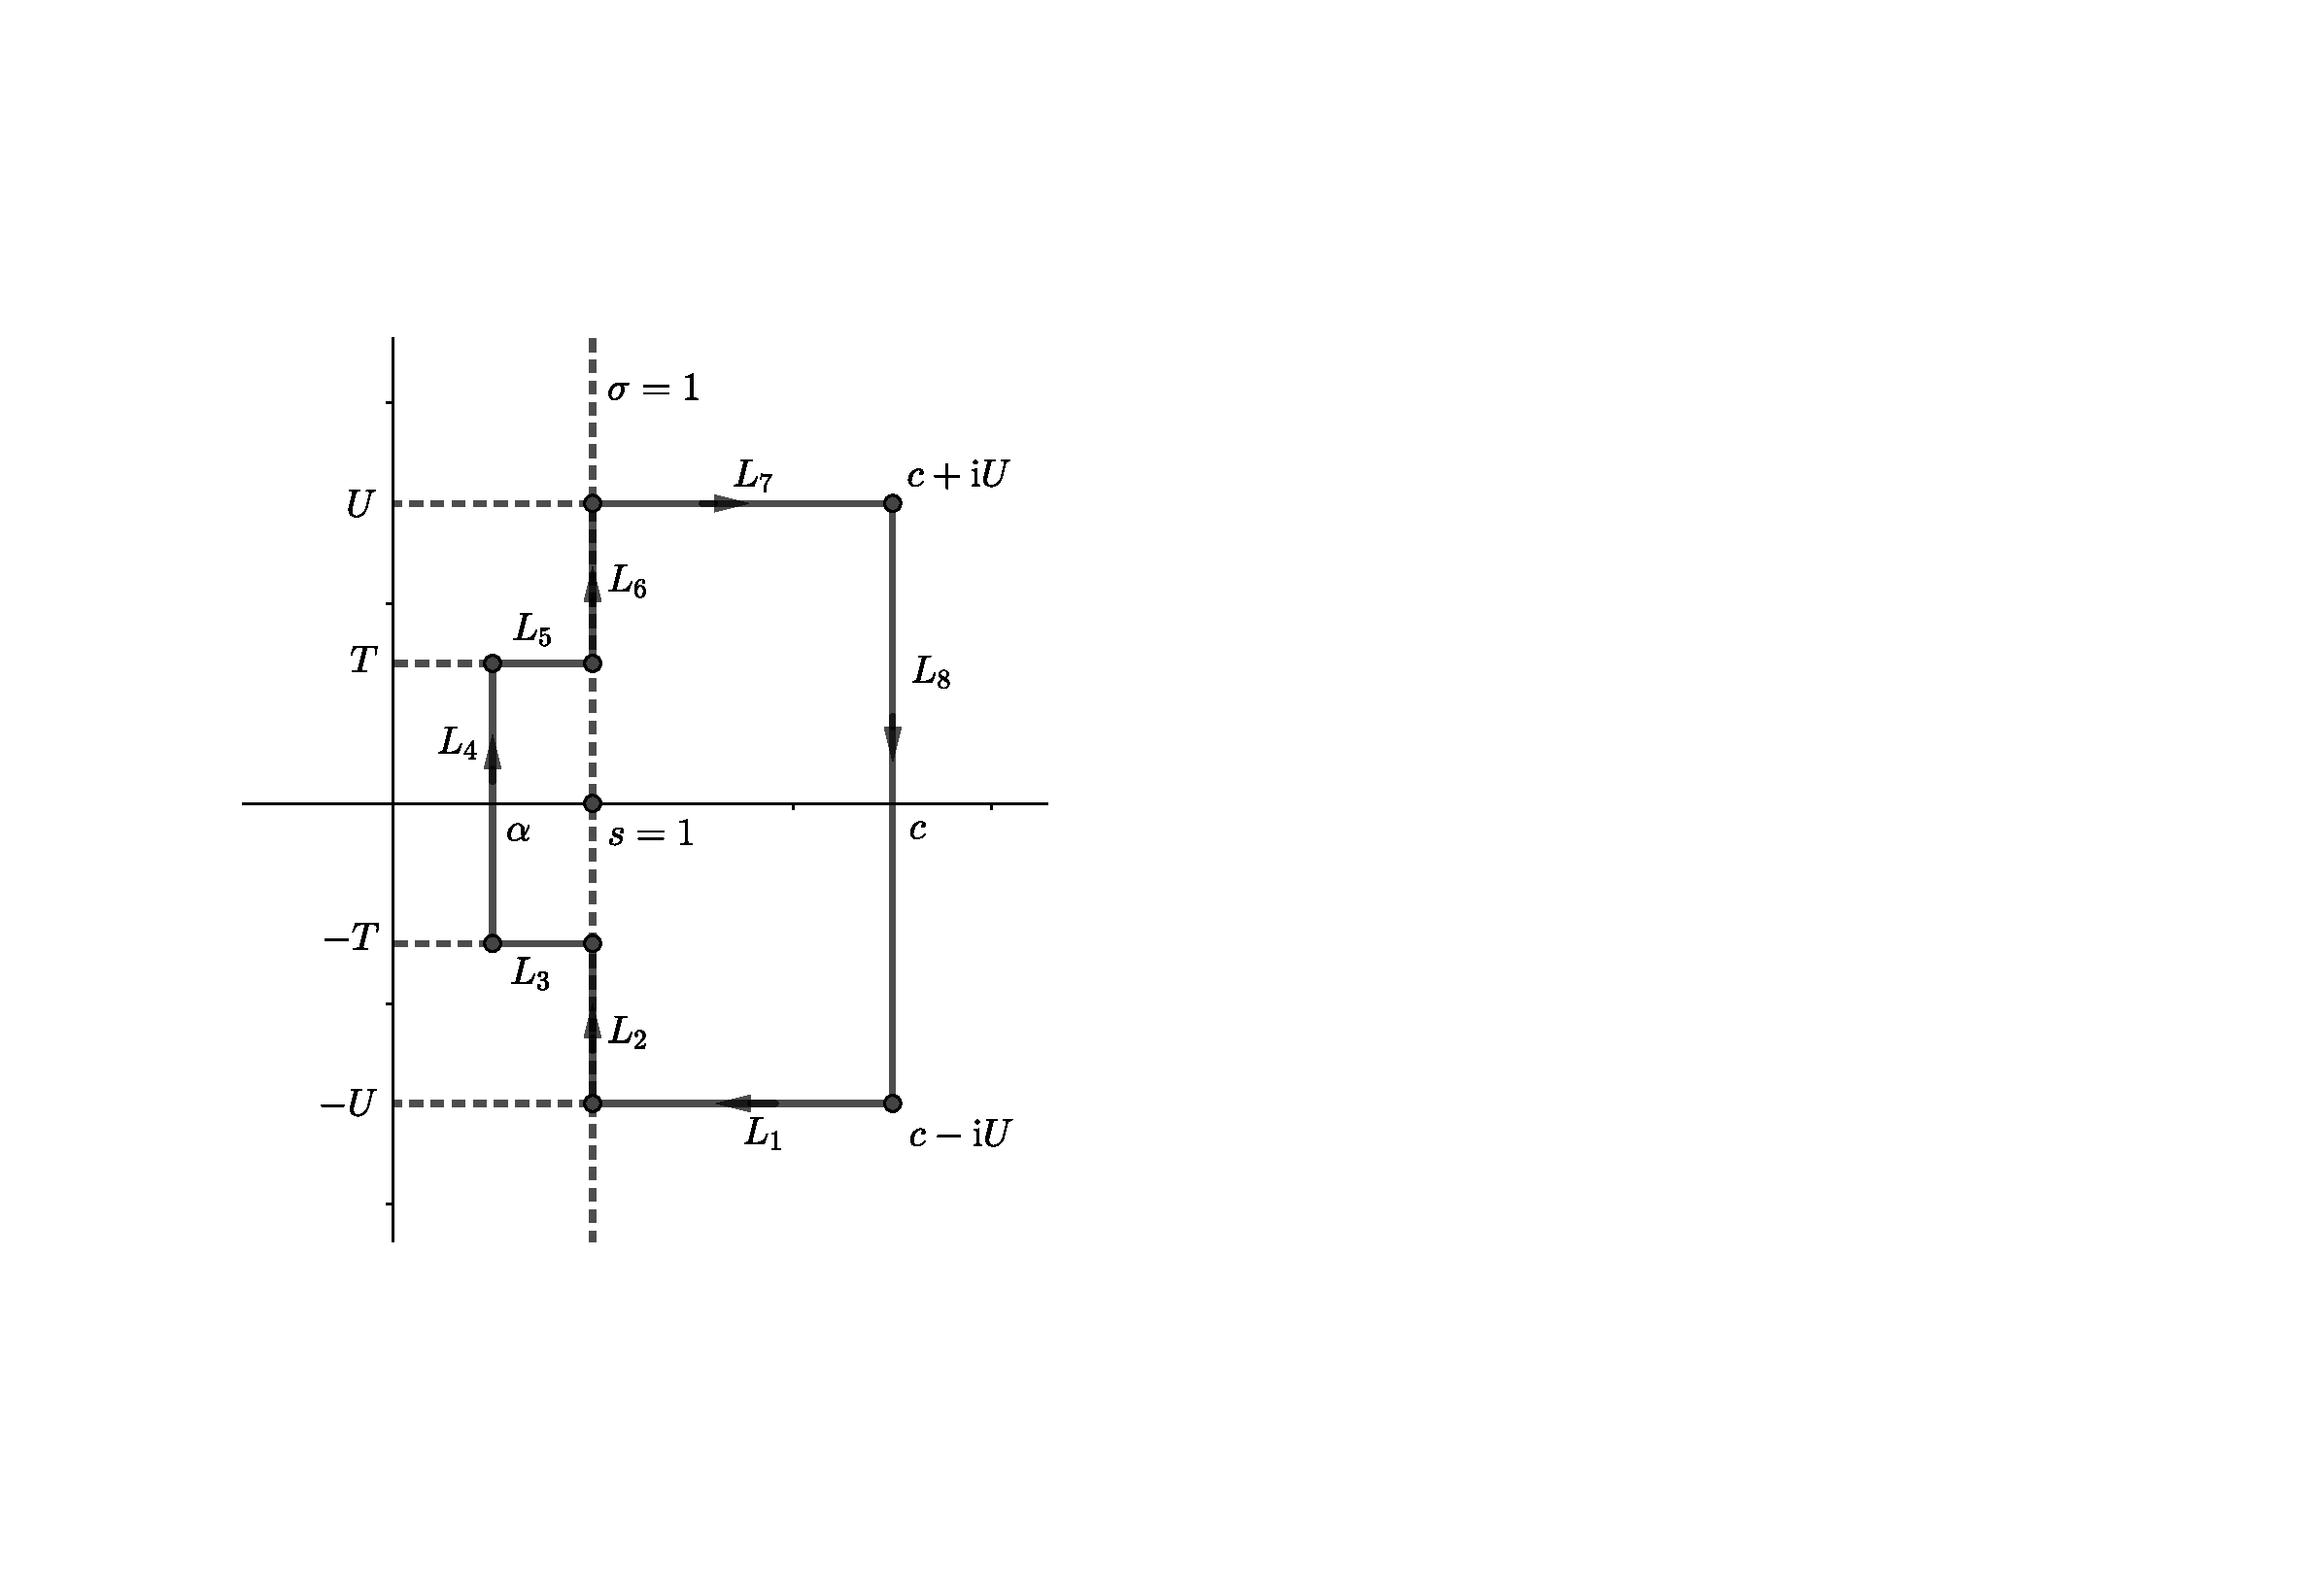
\includegraphics[scale=0.6]{PNT-last.pdf}
    \end{figure}

    其中
    \begin{equation*}
        \begin{cases}
            L_1=[c-\i u,1-\i u],&\quad L_2=[1-\i u,1-\i T],\\
            L_3=[1-\i T,\alpha-\i T],&\quad L_4=[\alpha+\i T,\alpha+\i T],\\
            L_5=[\alpha+\i T,1+\i T],&\quad L_6=[1+\i T, 1+\i u],\\
            L_7=[1+\i u, c+\i u],&\quad L_8=[c+\i u, c-\i u].
        \end{cases}
    \end{equation*}
    方向为顺时针方向(方便后面计算).

    由解析延拓后的$\zeta(s)$在半平面$\sigma > 0$上除去$s=1$外连续, 则存在包含曲线$\gamma$的区域$D$, 使$\zeta(s)$在$D$上无零点, 则$G(s)$是$D$上的亚纯函数, $s=1$为其唯一奇点.

    由\textbf{定理}\ref{thm-zeta}知
    \begin{equation*}
        \zeta(s) = \frac{A(s)}{B(s)} = \frac{\disp s-s(s-1)\int_1^{\infty}\frac{\{u\}}{u^{s+1}}\,\d u}{s-1}\quad(s\neq 1),
    \end{equation*}
    则$A(1) = 1, B(1) = 0, B'(1) = 1$, 于是
    \begin{equation*}
        G(s)x^{s-1} = \frac{x^{s-1}}{s(s+1)}\left(-\frac{\zeta'(s)}{\zeta(s)}\right) = \frac{B'(s)A(s)-A'(s)B(s)}{s(s+1)A(s)B(s)}x^{s-1} =: \frac{C(s)}{D(s)},
    \end{equation*}
    则$C(1)=B'(1)A(1) = 1,D(1) = 0, D'(1) = 2B'(1)A(1) = 2$, 所以$s=1$为$G(s)x^{s-1}$的一级极点, 且
    \begin{equation*}
        \res(G(s)x^{s-1},1)=\frac{C(1)}{D'(1)}=\frac{1}{2}.
    \end{equation*}

    由留数定理知
    \begin{equation*}
        \frac{1}{2\pi\i}\int_{c-\i U}^{c+\i U}G(s)x^{s-1}\,\d s=\sum_{j=1}^7\frac{1}{2\pi\i}\int_{L_j}G(s)x^{s-1}\,\d s +\frac{1}{2}.
    \end{equation*}
    记$I_j = \int_{L_j}G(s)x^{s-1}\,\d s$, 于是
    \begin{equation}\label{eq-end}
        \left|\frac{1}{2\pi\i}\int_{c-\i U}^{c+\i U}G(s)x^{s-1}\,\d s-\frac{1}{2}\right|\leq\sum_{j=1}^7\frac{1}{2\pi}\left|\int_{L_j}G(s)x^{s-1}\,\d s\right| = \sum_{j=1}^7\frac{|I_j|}{2\pi}.
    \end{equation}
    设$F'(s) = G(s)x^{s-1}$, 则$F(s)$在$D$上解析\footnote{这样的$F(s)$一定是存在且解析, 证明请见\cite{ref-complex}第四节命题4.12.}, 则$F(\ol{s}) = \ol{F(s)}$, 观察到
    \begin{equation*}
        \begin{aligned}
            |I_1| =&\ \left|\int_{c-\i U}^{1-\i U}F'(s)\,\d s\right| = |F(1-\i U) - F(c-\i U)| = |F(\ol{1+\i U})-F(\ol{c+\i U})|\\
            =&\ |\ol{F(1+\i U)}-\ol{F(c+\i U)}| = |F(1+\i U)-F(c+\i U)| = |I_7|
        \end{aligned}
    \end{equation*}
    类比地, 有$|I_2| = |I_6|,\ |I_3| = |I_5|$.

    设$M = \sup_{s\in L_3\cup L_4\cup L_5}|G(s)|$, 则
    \begin{equation*}
        \begin{aligned}
            |I_1| = |I_7| =&\ \left|\int_{1+\i U}^{c+\i U}G(s)x^{s-1}\,\d s\right| = \left|\int_1^cG(\sigma+\i U)x^{\sigma+\i U-1}\,\d \sigma\right|\\
            \leq&\ AU^{-\frac{3}{2}}\int_1^cx^{\sigma-1}\,\d \sigma\leq AU^{-\frac{3}{2}}\frac{x^{c-1}}{\log x},\\
            |I_2| = |I_6| =&\ \left|\int_{1+\i T}^{1+\i U}G(s)x^{s-1}\,\d s\right| = \left|\int_{T}^{U}G(1+\i t)x^{\i t}\,\d t\right| \leq \int_T^U|G(1+\i t)|\,\d t < \epsilon,\\
            |I_3| = |I_5| =&\ \left|\int_{\alpha+\i T}^{1+\i T}G(s)x^{s-1}\,\d s\right| = \left|\int_{\alpha}^1G(\sigma + \i T)x^{\sigma+\i T-1}\,\d \sigma\right|\\
            \leq&\ M\int_{\alpha}^1x^{\alpha-1}\,\d\sigma = \frac{M(1-x^{\alpha-1})}{\log x}\leq \frac{M}{\log x},\\
            |I_4|=&\ \left|\int_{\alpha-\i T}^{\alpha+\i T}G(s)x^{s-1}\,\d s\right|=\left|\int_{-T}^TG(\alpha+\i t)x^{\alpha+\i t-1}\,\d t\right|\leq 2TMx^{\alpha-1}.
        \end{aligned}
    \end{equation*}
    令$U\to \infty$, 则$I_1=I_7=0$, 由(\ref{eq-end})式可知
    \begin{equation*}
        \begin{aligned}
        \left|\frac{1}{2\pi \i}\int_{c-\i\infty}^{c+\i\infty}G(s)x^{s-1}\,\d s-\frac{1}{2}\right|\leq&\ \frac{1}{2\pi}(|I_2|+|I_3|+|I_4|+|I_5|+|I_6|)\\
        \leq&\ \frac{1}{2\pi}\left(\frac{2M}{\log x}+2\epsilon+2TMx^{\alpha-1}\right)\to 0\quad(x\to \infty).
        \end{aligned}
    \end{equation*}

    综上, 当$x\to\infty$时, $\frac{1}{2\pi\i}\int_{c-\i\infty}^{c+\i\infty}G(s)x^{s-1}\,\d s\sim \frac{1}{2}$.
\end{proof}

\clearpage
\begin{thebibliography}{99}
    \bibitem{ref-复变函数}方企勤. 复变函数教程[M]. 北京:北京大学出版社, 1996.12.
    \bibitem{ref-数分}陆亚明. 数学分析入门, 第二册[M]. 西安:西安交通大学出版社, 
    \bibitem{ref-three}Ciar´an O’Rourke. The prime number theorem: Analytic and elementary proofs[D]. Ollscoil na h-´Eireann, M´a Nuad, 2013.
    \bibitem{ref-complex}JOSEPH BAK, DONALD J. NEWMAN. Complex Analysis[M]. Springer-Verlag, 1995.
    \bibitem{ref-elementary}Atle Selberg. An Elementary Proof of the Prime-Number Theorem[C]. Annals of Mathematics, 1949, 305-313.
    \bibitem{ref-newman}Donald J. Newman. Simple Analytic Proof of the Prime Number Theorem[C]. American Mathematical Monthly, 1980, 693-696.
\end{thebibliography}

\end{document}

\iffalse
%%%% 表格模板 %%%%
\renewcommand\arraystretch{0.8} % 设置表格高度为原来的0.8倍
\begin{table}[!htbp] % table标准
    \centering % 表格居中
    \begin{tabular}{p{1cm}<{\centering}p{1cm}<{\centering}p{3cm}<{\centering}p{5cm}<{\centering}} % 设置表格宽度
    %\begin{tabular}{cccc}
        \toprule
        $x_i$ & $f[x_1]$ & $f[x_i, x_{i+1}]$ & $f[x_i, x_{i+1}, x_{i+2}]$ \\
        \midrule
        $x_0$ & $f(x_0)$ &                  &                          \\
        $x_0$ & $f(x_0)$ & $f'(x_0)$        &                          \\
        $x_0$ & $f(x_1)$ & $\frac{f(x_1)-f(x_0)}{x_1-x_0}$ & $\frac{f(x_1)-f(x_0)}{(x_1-x_0)^2}-\frac{f'(x_0)}{x_1-x_0}$\\
        \bottomrule
    \end{tabular}
\end{table}

%%%% 文字环绕图片, 标题加注释 %%%%
{ % 一般将文字环绕部分的图和文字, 用大括号括起来, 避免对文字外的格式发生影响
\begin{wrapfigure}[13]{r}{.5\linewidth} % 文字环绕行数为13行, 图片靠右 (l为靠左), 图片占0.5的行宽
    \centering
    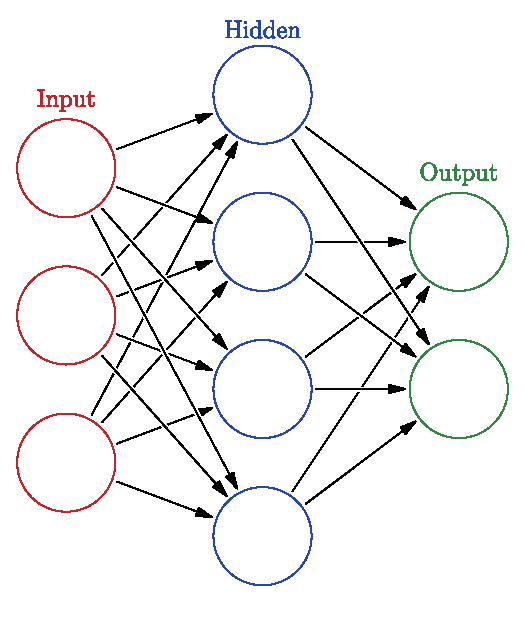
\includegraphics[scale=0.7]{neural_network.eps} % scale=0.7按比例缩放70%
    \caption{神经网络结构\protect\footnotemark[1]} % 记得加\protect, 设置1号脚标
    \label{figure-神经网络结构}
\end{wrapfigure}
\footnotetext[1]{图片来源: \url{https://en.wikipedia.org/wiki/File:Colored_neural_network.svg}}
文字文字
}

%%%% 普通图片, 标题加注释 %%%%
\begin{figure}[htbp] % h: 当前位置, t: 顶部, b: 底部, p: 浮动页, 这样组合指的是使用这个顺序进行排版
    \centering
    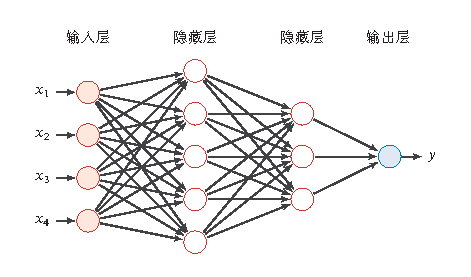
\includegraphics[scale=0.5]{前馈神经网络.eps}
    \caption{前馈神经网络\protect\footnotemark[1]}
    \label{figue-前馈神经网络}
\end{figure}
\footnotetext[1]{图片来源: 邱锡鹏, 神经网络与深度学习 \cite{ref-qxp}, 第92页}

%%%% 多组图 %%%%
    \begin{figure}[htbp]
        \centering
        \subfigure[迭代1次]  % 子图的标题
        {
            % 如果一行放三个图改成0.3\linewidth即可
            \begin{minipage}[b]{.45\linewidth}  % 0.45排版行距, 即一行放2个图, 一行放不下就换行
                \centering
                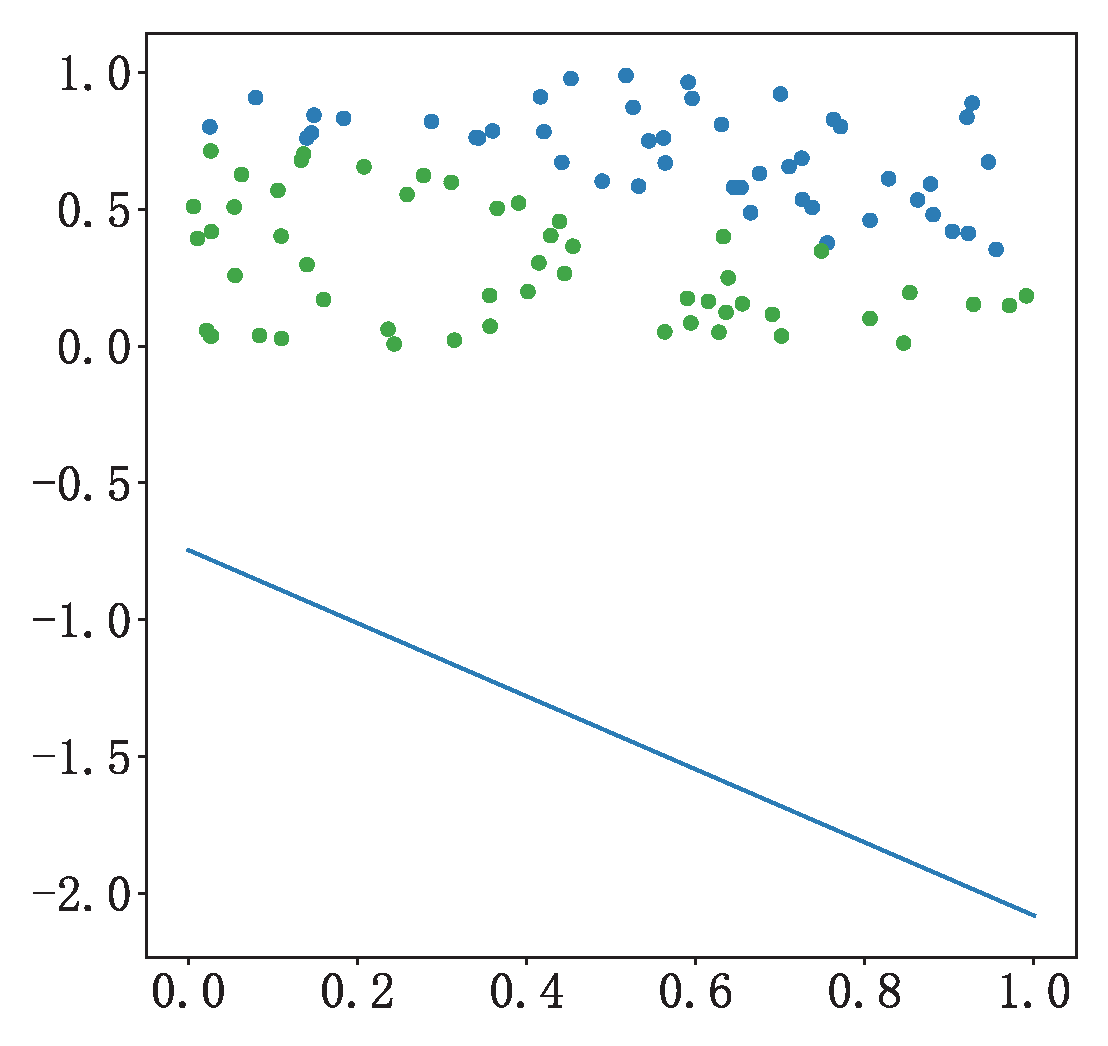
\includegraphics[scale=0.35]{1.eps}
            \end{minipage}
        }
        \subfigure[迭代100次]
        {
            \begin{minipage}[b]{.45\linewidth}
                \centering
                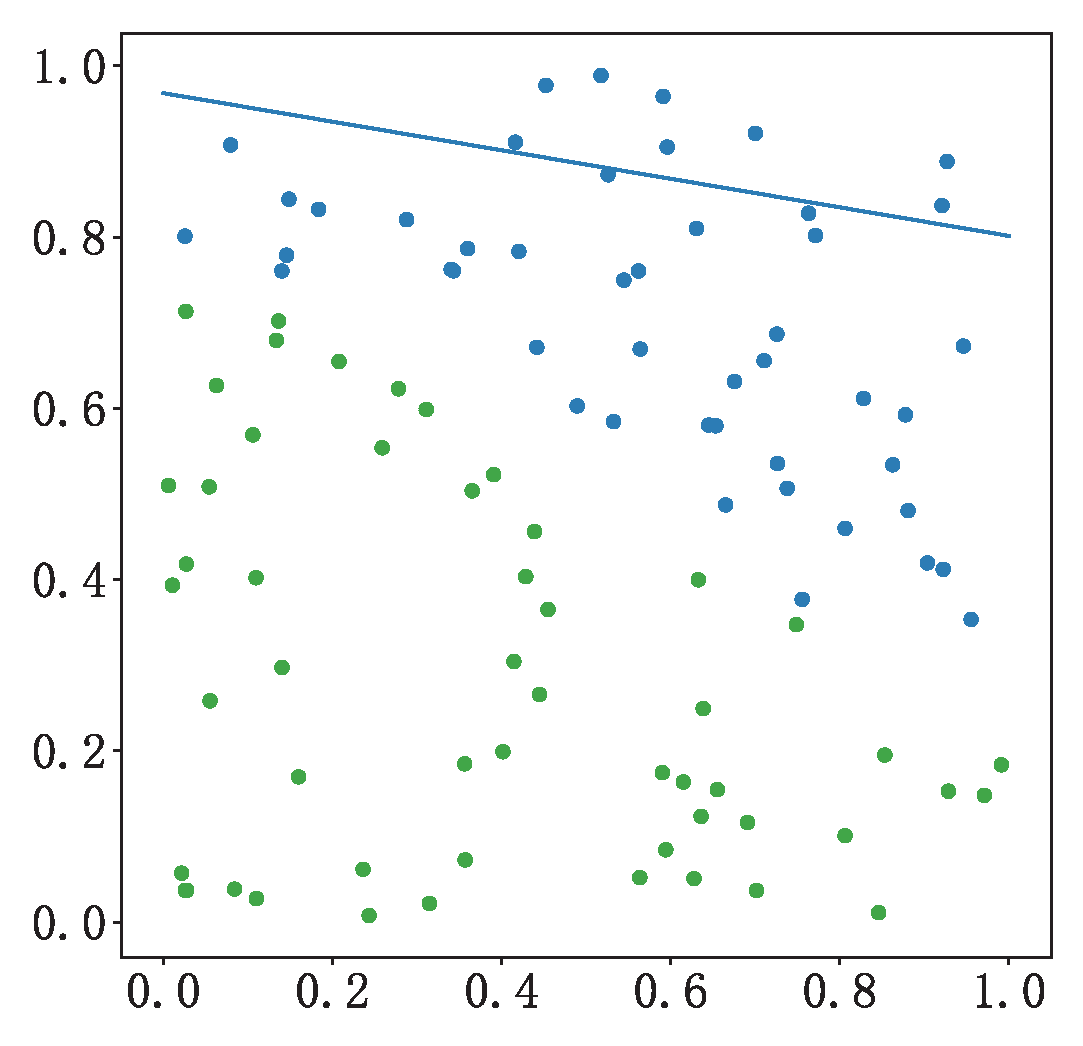
\includegraphics[scale=0.35]{100.eps}
            \end{minipage}
        }
        \subfigure[迭代500次]
        {
            \begin{minipage}[b]{.45\linewidth}
                \centering
                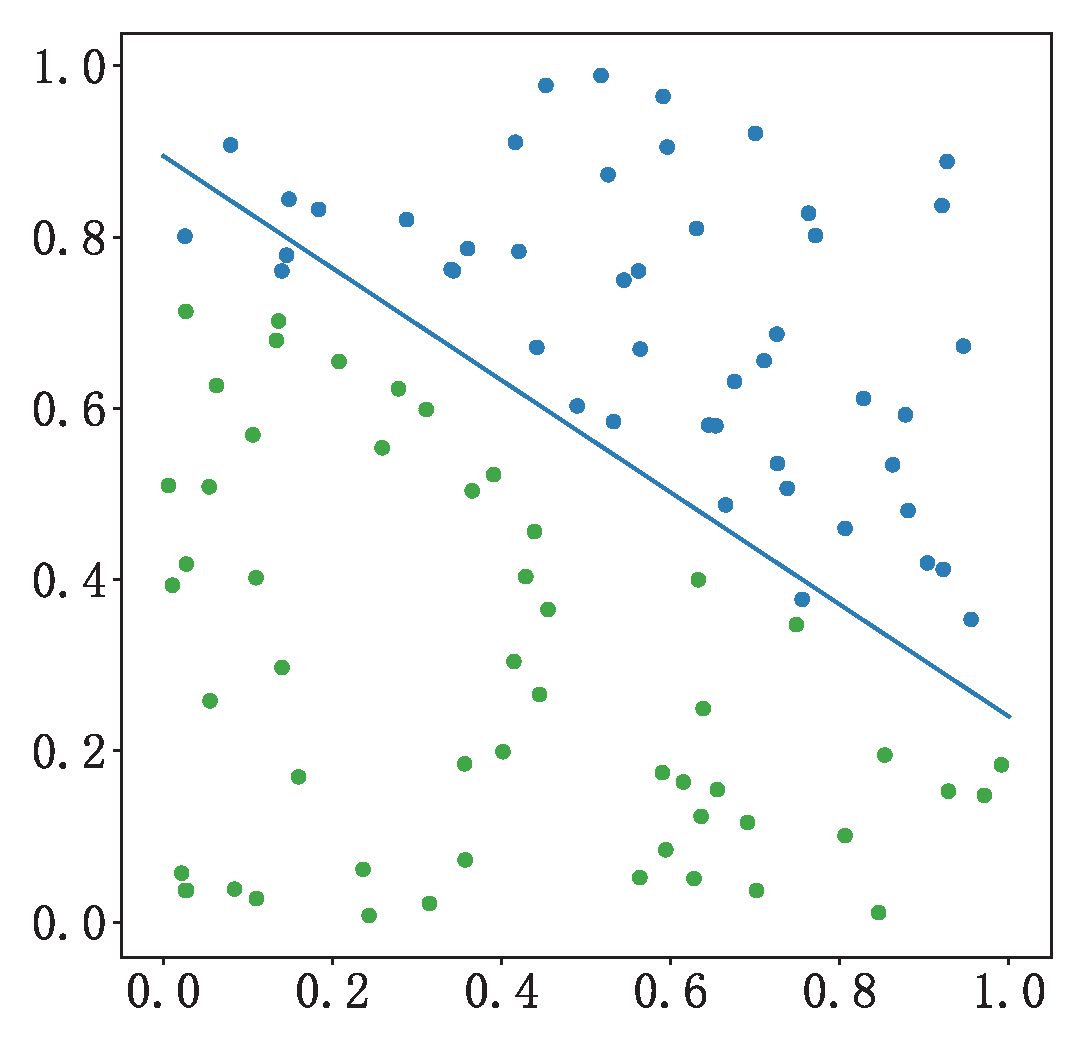
\includegraphics[scale=0.35]{500.eps}
            \end{minipage}
        }
        \subfigure[迭代2000次]
        {
            \begin{minipage}[b]{.45\linewidth}
                \centering
                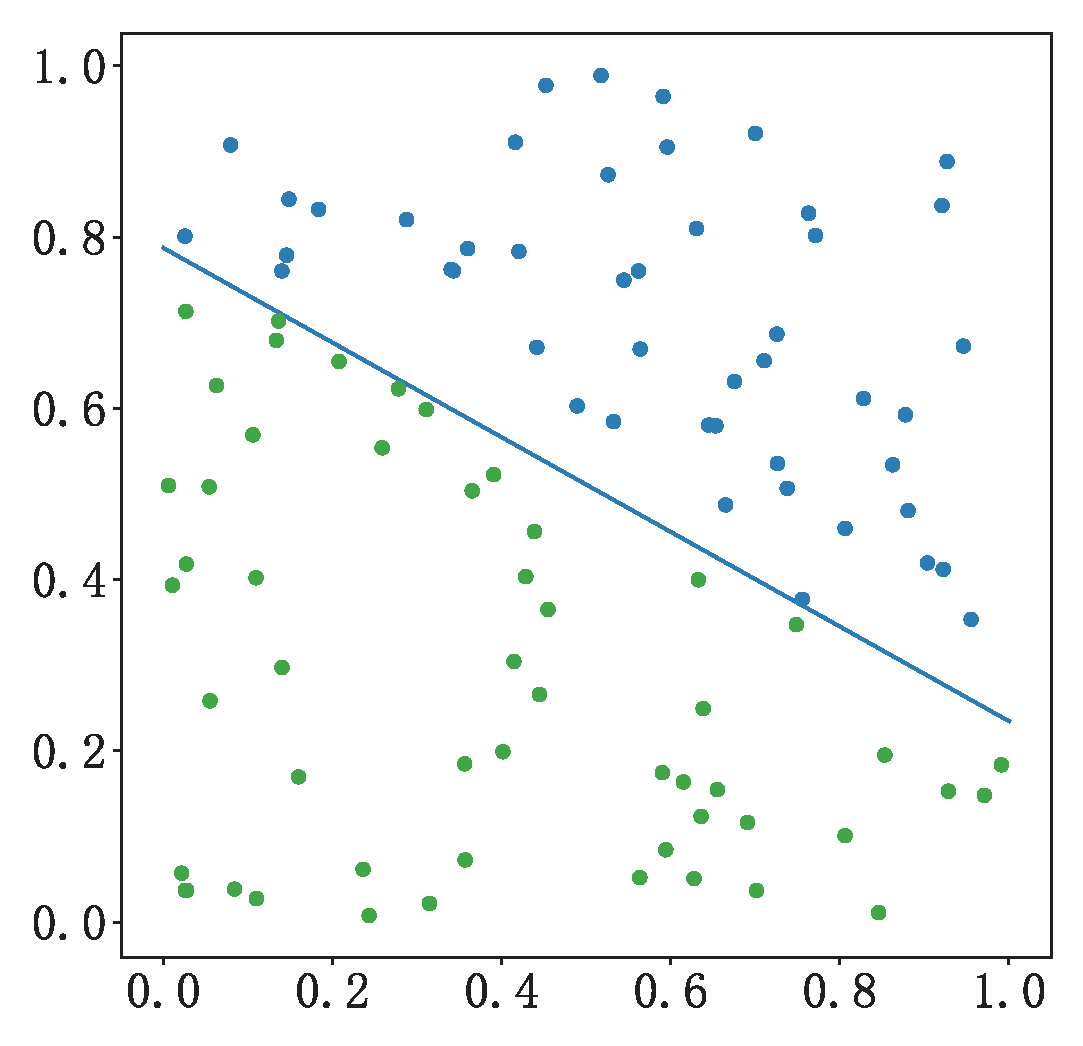
\includegraphics[scale=0.35]{2000.eps}
            \end{minipage}
        }
        \caption{迭代过程图}
        \label{figure-迭代过程图}
    \end{figure}
\fi
